% Options for packages loaded elsewhere
\PassOptionsToPackage{unicode}{hyperref}
\PassOptionsToPackage{hyphens}{url}
%
\documentclass[
]{book}
\title{Silbiger Lab Mesocosm User Manual}
\author{Dr.~Nyssa Silbiger and Danielle Barnas}
\date{2022-03-01}

\usepackage{amsmath,amssymb}
\usepackage{lmodern}
\usepackage{iftex}
\ifPDFTeX
  \usepackage[T1]{fontenc}
  \usepackage[utf8]{inputenc}
  \usepackage{textcomp} % provide euro and other symbols
\else % if luatex or xetex
  \usepackage{unicode-math}
  \defaultfontfeatures{Scale=MatchLowercase}
  \defaultfontfeatures[\rmfamily]{Ligatures=TeX,Scale=1}
\fi
% Use upquote if available, for straight quotes in verbatim environments
\IfFileExists{upquote.sty}{\usepackage{upquote}}{}
\IfFileExists{microtype.sty}{% use microtype if available
  \usepackage[]{microtype}
  \UseMicrotypeSet[protrusion]{basicmath} % disable protrusion for tt fonts
}{}
\makeatletter
\@ifundefined{KOMAClassName}{% if non-KOMA class
  \IfFileExists{parskip.sty}{%
    \usepackage{parskip}
  }{% else
    \setlength{\parindent}{0pt}
    \setlength{\parskip}{6pt plus 2pt minus 1pt}}
}{% if KOMA class
  \KOMAoptions{parskip=half}}
\makeatother
\usepackage{xcolor}
\IfFileExists{xurl.sty}{\usepackage{xurl}}{} % add URL line breaks if available
\IfFileExists{bookmark.sty}{\usepackage{bookmark}}{\usepackage{hyperref}}
\hypersetup{
  pdftitle={Silbiger Lab Mesocosm User Manual},
  pdfauthor={Dr.~Nyssa Silbiger  and Danielle Barnas},
  hidelinks,
  pdfcreator={LaTeX via pandoc}}
\urlstyle{same} % disable monospaced font for URLs
\usepackage{longtable,booktabs,array}
\usepackage{calc} % for calculating minipage widths
% Correct order of tables after \paragraph or \subparagraph
\usepackage{etoolbox}
\makeatletter
\patchcmd\longtable{\par}{\if@noskipsec\mbox{}\fi\par}{}{}
\makeatother
% Allow footnotes in longtable head/foot
\IfFileExists{footnotehyper.sty}{\usepackage{footnotehyper}}{\usepackage{footnote}}
\makesavenoteenv{longtable}
\usepackage{graphicx}
\makeatletter
\def\maxwidth{\ifdim\Gin@nat@width>\linewidth\linewidth\else\Gin@nat@width\fi}
\def\maxheight{\ifdim\Gin@nat@height>\textheight\textheight\else\Gin@nat@height\fi}
\makeatother
% Scale images if necessary, so that they will not overflow the page
% margins by default, and it is still possible to overwrite the defaults
% using explicit options in \includegraphics[width, height, ...]{}
\setkeys{Gin}{width=\maxwidth,height=\maxheight,keepaspectratio}
% Set default figure placement to htbp
\makeatletter
\def\fps@figure{htbp}
\makeatother
\setlength{\emergencystretch}{3em} % prevent overfull lines
\providecommand{\tightlist}{%
  \setlength{\itemsep}{0pt}\setlength{\parskip}{0pt}}
\setcounter{secnumdepth}{5}
\usepackage{booktabs}
\usepackage{amsthm}
\makeatletter
\def\thm@space@setup{%
  \thm@preskip=8pt plus 2pt minus 4pt
  \thm@postskip=\thm@preskip
}
\makeatother
\ifLuaTeX
  \usepackage{selnolig}  % disable illegal ligatures
\fi
\usepackage[]{natbib}
\bibliographystyle{apalike}

\begin{document}
\maketitle

{
\setcounter{tocdepth}{1}
\tableofcontents
}
\hypertarget{summary}{%
\chapter{Summary}\label{summary}}

This manual describes the design, operation, and maintenance of the Silbiger Lab mesocosm system, located in the loading bay between Citrus Hall and Eucalyptus Hall at California State University, Northridge, funded and operated by Dr.~Nyssa Silbiger.

Requests for use of the mesocosm system can be made \href{https://docs.google.com/forms/d/1LCZG39k8dJmIDLb5l6XBP8-Ow2yxawrKlUB2wUDesqg/edit}{here}

\hypertarget{contacts}{%
\chapter{Contacts}\label{contacts}}

\begin{longtable}[]{@{}
  >{\raggedright\arraybackslash}p{(\columnwidth - 6\tabcolsep) * \real{0.20}}
  >{\raggedright\arraybackslash}p{(\columnwidth - 6\tabcolsep) * \real{0.28}}
  >{\raggedright\arraybackslash}p{(\columnwidth - 6\tabcolsep) * \real{0.32}}
  >{\raggedright\arraybackslash}p{(\columnwidth - 6\tabcolsep) * \real{0.20}}@{}}
\toprule
\begin{minipage}[b]{\linewidth}\raggedright
Name
\end{minipage} & \begin{minipage}[b]{\linewidth}\raggedright
Involvement
\end{minipage} & \begin{minipage}[b]{\linewidth}\raggedright
Contact Information
\end{minipage} & \begin{minipage}[b]{\linewidth}\raggedright
Notes
\end{minipage} \\
\midrule
\endhead
Nyssa Silbiger & System Design Asst. Professor, CSUN & \href{mailto:nyssa.silbiger@csun.edu}{\nolinkurl{nyssa.silbiger@csun.edu}} 818-677-4427 & \\
Jennifer Fields & Silbiger Lab Tech, CSUN & \href{mailto:jennifer.fields.855@my.csun.edu}{\nolinkurl{jennifer.fields.855@my.csun.edu}} & \\
Danielle Barnas & System Installation and Maintenance Silbiger Lab Graduate Student, CSUN & \href{mailto:danielle.barnas@csun.edu}{\nolinkurl{danielle.barnas@csun.edu}} & \\
Louis Dang & Systems Engineer & \href{mailto:louis@aqualogicinc.com}{\nolinkurl{louis@aqualogicinc.com}} & \href{http://www.aqualogicinc.com}{www.aqualogicinc.com} \\
Science Shop & CSUN College of Science and Math Machine Shop & 818-677-3055 & Location: EH 2014 Available M-Th 0600-1630 \href{http://www.csun.edu/science-mathematics/science-shop}{www.csun.edu/Science-Shop} \\
Wendy Dunbarr & Support Technician, CSUN Stockroom & \href{mailto:wendy.dunbarr@csun.edu}{\nolinkurl{wendy.dunbarr@csun.edu}} 818-677-2056 & Location: CH 5108 \\
Perry Martin & Supervising Plumber, PPM & \href{mailto:perry.martin@csun.edu}{\nolinkurl{perry.martin@csun.edu}} 818-677-2222 (PPM) 818-677-2237 & \\
Will Moran & Network Engineer, CSUN IT & \href{mailto:will.moran@csun.edu}{\nolinkurl{will.moran@csun.edu}} 818-677-6273 & \\
Willy Martinez & Lead Electrician, PPM Electric Shop & \href{mailto:willy.martinez@csun.edu}{\nolinkurl{willy.martinez@csun.edu}} 818-677-6273 & \\
Neptune Systems & Apex Support Team & \href{mailto:support@neptunesystems.com}{\nolinkurl{support@neptunesystems.com}} & \href{http://www.neptunesystems.com}{www.neptunesystems.com} \\
Dickson Lab & Seawater CO2 CRMs & \href{mailto:co2crms@ucsd.edu}{\nolinkurl{co2crms@ucsd.edu}}, 858-534-2582 & Certified Reference Materials Laboratory Scripps Institution of Oceanography University of California, San Diego Andrew Dickson 2350 Downwind way Room 15 La Jolla, CA 92037 \\
\bottomrule
\end{longtable}

\hypertarget{system-details}{%
\chapter{System Details}\label{system-details}}

\textbf{Contents}\\
- \protect\hyperlink{Aquaria_System_Item_List}{\textbf{Aquaria System Item List}}\\
- \protect\hyperlink{Filtration_and_Recirculation_System}{\textbf{Filtration and Recirculation System}}\\
- \protect\hyperlink{System_Operation_Parameters}{\textbf{System Operational Parameters}}\\
- \protect\hyperlink{Apex_Connection_Series}{\textbf{Apex Connection Series}}\\
- \protect\hyperlink{EB832_Outlet_Connections}{\textbf{EB832 Outlet Connections}}\\
- \protect\hyperlink{Water_Flow_Operation}{\textbf{Water Flow Operation}}

\textbf{Aquaria System Component List}

\begin{itemize}
\tightlist
\item
  Experimental Tanks (21.25'' x 12.5'' x 13.5''H, 14.37 gal) - Per tank:

  \begin{itemize}
  \tightlist
  \item
    1 Submersible powerhead pump (\href{https://github.com/SilbigerLab/Mesocosm_User_Manual/blob/master/Manuals/Hydor_Nano_Pump.pdf}{Hydor Nano Koralia 240 powerhead})\\
  \item
    1 200 W Heater (\href{https://github.com/SilbigerLab/Mesocosm_User_Manual/blob/master/Manuals/Hydor_Heater.pdf}{Hydor aquarium heater})\\
  \item
    1 Light (\href{https://github.com/SilbigerLab/Mesocosm_User_Manual/blob/master/Manuals/Apex_Halo.pdf}{Halo Basic M-110})\\
  \item
    1 Temperature probe (Apex)\\
  \item
    1 pH probe (Apex)\\
  \item
    1 Solenoid valve for pH (Apex)\\
  \item
    1 air stone and tubing to bubble CO2\\
  \item
    3 Flow sensors (Apex, FS-25 1/4'' fitting, flow rates from 3-12 GPH (12-45 LPH))\\
  \item
    1 Main Supply line: ``N''\\
  \item
    1 Solenoid Supply line: ``S''\\
  \item
    1 Drain line: ``D''\\
  \item
    1 Overflow drain port\\
  \item
    1 Controlled drain port (PVC \textasciitilde{} 1/2 tank height)\\
  \item
    1 Gate valve (solenoid for water inflow)\\
  \item
    1 VDM (\href{https://github.com/SilbigerLab/Mesocosm_User_Manual/blob/master/Manuals/VDM_manual.pdf}{Apex Variable Dimming Module}, 1 unit for 2 tanks)\\
  \item
    1 FMM (\href{https://www.neptunesystems.com/getstarted/fmk/}{Apex Fluid Metering Module})\\
  \item
    1 PM1 (\href{https://github.com/SilbigerLab/Mesocosm_User_Manual/blob/master/Manuals/PM1_manual.pdf}{Apex Probe Module 1})\\
  \end{itemize}
\item
  Experimental Tanks - Per Apex, Rack of 4 tanks:

  \begin{itemize}
  \tightlist
  \item
    1 Base Unit (\href{https://github.com/SilbigerLab/Mesocosm_User_Manual/blob/master/Manuals/Apex_Comprehensive_Reference_Manual.pdf}{Apex} processing unit, 1 unit for 4 tanks)\\
  \item
    2 EB832 (\href{https://github.com/SilbigerLab/Mesocosm_User_Manual/blob/master/Manuals/EB832_Guide.pdf}{Apex 8-outlet EnergyBar}, 1 unit for 2 tanks)\\
  \item
    1 Conductivity probe (Apex)\\
  \end{itemize}
\item
  1 CO2 regulator valve (\href{https://github.com/SilbigerLab/Mesocosm_User_Manual/blob/master/Manuals/Tunze_CO2_Regulator.pdf}{Tunze pH Controller Set, pressure reducing valve 7077/3})\\
\item
  1 Industrial Grade Carbon Dioxide, \href{https://www.airgas.com/product/Gases/Industrial-Application-Gases/Carbon-Dioxide---Industrial/p/CD\%2050}{50 pound cylinder}
\end{itemize}

\textbf{Filtration and Recirculation} \href{https://github.com/SilbigerLab/Mesocosm_User_Manual/blob/master/Manuals/Filtration_Skid_Build_Package.pdf}{\textbf{System}} \textbf{Component List}

\begin{itemize}
\tightlist
\item
  Sump (66.25'' x 31.5'' x 21''H)\\
\item
  Chiller and Heat Pump (\href{https://github.com/SilbigerLab/Mesocosm_User_Manual/blob/master/Manuals/AquaLogic_Chiller.pdf}{AquaLogic Multi-Temp and Titan Series})\\
\item
  1 PM1 (\href{https://github.com/SilbigerLab/Mesocosm_User_Manual/blob/master/Manuals/PM1_manual.pdf}{Apex Probe Module 1})\\
\item
  1 Temperature probe (Apex)\\
\item
  1 pH probe (Apex)
\item
  Water pump (\href{https://github.com/SilbigerLab/Mesocosm_User_Manual/blob/master/Manuals/Complete_Cascade.pdf}{PerformancePro Cascade pump})\\
\item
  UV Sterilizer (Comet Series 95 Watt Lamp)\\
\item
  2 PhosBan chemical filter (\href{https://github.com/SilbigerLab/Mesocosm_User_Manual/blob/master/Manuals/Phosban_Reactor.pdf}{PhosBan Reactor 550})\\
\item
  2 Air compressors\\
\item
  10 Airstones and tubing (4 units on one phosban reactor, 6 units on the other)\\
\item
  3 Mesh filters (AquaLogic, 50 microns mesh size)\\
\item
  3 Carbon filter cells with mesh casing (AquaLogic, CF28AC,28in, ActC)\\
\item
  4 Blue high density mesh filters (Matala Filter Media)\\
\item
  4 Black low density mesh filters (Matala Filter Media)
\end{itemize}

\textbf{System Operational Parameters}

\begin{itemize}
\tightlist
\item
  This is a closed loop system where water from each individual tank will recirculate back to a main holding reservoir (sump).\\
\item
  Normal High Tide operating water level is approximately 12.5''H for a total water volume of 14.37 gal per tank (total of 287.4 gal to fill the available 20 tanks).\\
\item
  Normal Low Tide operating water level is approximately 4''H for a total water volume of 4.60 gal per tank (92.0 gal total for the 20-tank-system).\\
\item
  Excess water drained to the sump at low tide is 9.77 gal per tank (195.4 gal total for the 20-tank-system).\\
\item
  Normal sump operating water level is 7'' water in the filter cell compartment, about 2 inches above the three carbon filters. The sump at this level has an approximate volume of 82.32 gal. Sump freeboard volume (max before overflow) is 107.39 gal.\\
\item
  Secondary sump available volume is 250 gal. To operate from a High Tide water level to a Low Tide water level, excess water must be redirected to the secondary sump to accomodate the excess volume (see below).\\
\item
  Aquaria drain pipe is in line with a 30 gal sump pump, which will draw water from the aquaria drain line and pump water to the sump.\\
\item
  Outflow water from the tanks feeds down to the outside underground sump pump, then into to the filtration system inside the Citrus Hall Field Room.\\
\item
  Water pumped into the Field Room flows through three 50um bag filters and eight matala mesh filters before overflowing into the main holding reservoir. Reservoir water is pumped through three carbon filters, a UV sterilizer, and chiller, then either back into the holding reservoir or to the tanks.

  \begin{itemize}
  \tightlist
  \item
    Biological and Mechanical Filtration: Water from the Mesocosm tanks is pumped into the sump while passing through three 50um bag filters and eight matala mesh filters (high and low density) to pick up debris. These filters have an accumulated biofilm to biologically filter the water before entering the sump and returning to the tanks.
  \item
    Chemical and Mechanical Filtration: Water in the sump is pulled through three carbon filters with mesh filter sleeves and pumped into a UV sterilizer before entering the sump and returning to the tanks.\\
  \end{itemize}
\item
  Water directed toward the tanks has two potential inflow ports (one constant flow and one controlled by a solenoid) and two potential outflow ports (one overflow port and one controlled by a manual open/close needle valve to adjust tank volume)\\
\item
  Sump is in line with a secondary holding tank for sump overflow at Low Tide.

  \begin{itemize}
  \tightlist
  \item
    195.4 gal returning to sump in a Low Tide scenario will be split between the main and secondary sumps so that water level is the same in each.\\
  \end{itemize}
\item
  \textbf{Total system water volume should not exceed 390 gal - ideal water volume for this scenario is 375 gal total throughout the system}
\item
  Flow rate for each tank can be maintained at \textasciitilde2-6 GPH (See \href{07-tidal_manipulation.md}{Tidal Manipulation} for specific flow rates).\\
\item
  Chiller is plumbed inline with the \href{https://github.com/SilbigerLab/Mesocosm_User_Manual/blob/master/Manuals/Filtration_Skid_Build_Package.pdf}{filtration skid}, which includes mechanical/biological filtration as well as UV sterilization (chemical filtration).\\
\item
  One main pump recirculates the water flow throughout the experimental tanks and the main holding reservoir.\\
\item
  Each tank has an immersion heater that allows tank temperatures to be set \textasciitilde15 degF (8.3 degC) above the main holding tank reservoir.

  \begin{itemize}
  \tightlist
  \item
    \textbf{Note: The tank needs to have low flow or be static in order to initially heat up to desired temperatures \emph{much} higher than the sump. Once the temperature has been reached in the system, then flow can be set to the normal operating rate.}\\
  \end{itemize}
\item
  A small sumbersible powerhead in each tank provides water circulation throughout the tank.\\
\item
  Each tank has (2) water supply lines, each with (1) Neptune Systems flow sensor and (1) needle valve for manual flow rate control, and (1) gate solenoid valve in line with (1) supply line for programmable tidal effect. Each tank also has (2) drain lines with (1) flow sensor in line with (1) needle valve for outgoing flow rate control, and (1) `overflow' line for maintaining maximum tank volume. Incoming and outgoing flow rates have to be manually adjusted for tidal effect.\\
\item
  Flow metered water lines

  \begin{itemize}
  \tightlist
  \item
    N: Main supply
  \item
    S: Solenoid-controlled supply
  \item
    D: Drain\\
  \end{itemize}
\item
  Tidal effect

  \begin{itemize}
  \tightlist
  \item
    outgoing tide: incoming flow rate (N + S) is lower than outgoing flow rate (D).
  \item
    incoming tide: incoming flow rate (N + S) is greater than outgoing flow rate (D).
  \item
    Note: The tank will not be completely empty during low tide events to prevent the recirculating powerhead from running dry.\\
  \end{itemize}
\item
  Each tank has (1) CO2 supply line with an airstone connected to (1) Neptune Systems solenoid valve to control the lowering and maintenance of pH in tanks.\\
\item
  CO2 scrubber comprised of (1) or (2) air compressors connected to (1) or (2) Phosban Reactors will bubble out CO2 from the sump water to bring up pH to ambient or near-ambient conditions in the holding reservoir to supply to the tanks.\\
\item
  Each tank has individual LED lighting, which can be controlled for white or blue light for natural daily light cycles or some other program.\\
\item
  Certain tank conditions can be controlled via Neptune Systems Apex Controllers. Each Apex controls (4) tanks.

  \begin{itemize}
  \tightlist
  \item
    Controllable parameters are: pH, temperature, tidal effect (S flow into the tank), and lighting.\\
  \end{itemize}
\item
  Certain tank conditions can be monitored via Neptune Systems Apex Controllers. Each Apex monitors and records data for (4) tanks.

  \begin{itemize}
  \tightlist
  \item
    Monitored parameters include: pH, temperature, salinity, flow rates, relative light intensity, and the status of any set program (whether a unit is On of Off at any given time based on the program set)
  \end{itemize}
\end{itemize}

\textbf{Apex Connection Series}

\begin{itemize}
\tightlist
\item
  Each EnergyBar connects to the Base Unit with an AquaBus cable via the AquaBus Ports for power. (2) EB832 units connect to (1) Base Unit.\\
\item
  Each CO2 Solenoid valve connects to the EnergyBar via the DC24 Accessory Port on the side of the EB832. (2) Solenoid valves connect in (1) EB832.\\
\item
  (1)PM1 connects to (1) EnergyBar with an AquaBus cable via the AquaBus Ports, and all PM1 modules connect in series with each other for power.\\
\item
  VDM connects to the last PM1 in series with an AquaBus cable via the AquaBus Ports for power.\\
\item
  Temperature probes connect to the PM1 Temp Port or the Base Unit Temp Port. (1) Temperature probe in each PM1, and (1) Temperature probe in the Base Unit.\\
\item
  pH probes connect to the PM1 pH/ORP Port or the Base Unit pH/ORP Port. Push the BNC female connector of the probe on to the male connector and turn 1/4 turn clockwise to lock the connector in place. (1) pH probe in each PM1, and (1) pH probe in the Base Unit.\\
\item
  \href{https://github.com/SilbigerLab/Mesocosm_User_Manual/tree/394a3f7d9fed8765e4152f9fdd11d00a2ea87a93/Manuals/HALO_Quick_Start_Guide.pdf}{Halo light} connects to the VDM or Base Unit via the V1/V2 or V3/V4 Port. (2) Light connections in the VDM and (2) Light connections in the Base Unit.\\
\item
  (1)FMM connects to (1) EnergyBar (whichever EB832 is not powering the PM1 modules) with an AquaBus cable via the AquaBus Ports, and all FMM connect in series with each other for power.\\
\item
  (3)Flow sensors connect to each FMM via (3) of the numbered ports.
\end{itemize}

\textbf{EB832 Outlet Connections}

Note: Each horizontal row on an EB832 corresponds to one tank, yielding 4 outlets per aquarium. Current outlet order, left to right:

\begin{enumerate}
\def\labelenumi{\arabic{enumi}.}
\tightlist
\item
  200W Heater
\item
  Hydor Powerhead
\item
  Water supply line ``S'' Solenoid
\item
  Halo Light
\end{enumerate}

\textbf{Water Flow Operation}

\begin{itemize}
\tightlist
\item
  Flow from the filtration sump to the mesocosm tanks

  \begin{itemize}
  \tightlist
  \item
    Water from the chiller can be directed either back into the sump or to the mesocosm tanks or both simultaniously.\\
  \item
    The bypass valve is used to regulate the line pressure going back to the mesocosm tanks. The more closed, the higher the pressure in the line, and the more open, the lower the pressure.\\
  \item
    It is recommeded you maintain partial flow to the sump to maintain circulation within the sump and to not overwhelm the tanks with more water pressure than they can handle, depending on your flow rates in.\\
  \item
    Multiple valaves in line can be used to regulate the flow through the filtration system, though the chiller has a safety flow switch that requires a minimum flow rate for the chiller to operate.\\
  \item
    Minimize flow through the filtration system if you want to increase residence time of water through the UV sterilizer.\\
  \end{itemize}
\item
  Flow from the mesocosm tanks to the filtration sump

  \begin{itemize}
  \tightlist
  \item
    Water from the tanks drains to an outdoor underground 30 gal compartment, which will automatically pump water out when a certain water level is reached (about 15 gal). This water can be directed either back into the sump, or if you intend to drain water in the event of a water change or the end of an experiment, water can be directed to a drain port.
  \end{itemize}
\item
  Overflow from sump to secondary containment

  \begin{itemize}
  \tightlist
  \item
    When mesocosm water level falls from a high tide to low tide sequence, more water will drain to the sump than what the main sump can individually hold. Excess water can be redirected from the sump (S1) to the secondary containment (S2) by opening the S2 inflow t-valve (allows simultaneous flow of filtered, chilled water to both S2 and the mesocosm tanks), and an exchange t-valve (allows for continuous flow between S1 and S2).
  \end{itemize}
\end{itemize}

\hypertarget{inventory}{%
\chapter{Inventory}\label{inventory}}

\textbf{Contents}\\
- \protect\hyperlink{Mesocosm_Tanks}{\textbf{Mesocosm Tanks}}\\
- \protect\hyperlink{Filtration}{\textbf{Filtration}}\\
- \protect\hyperlink{Additional_Items}{\textbf{Additional Items}}

\textbf{Mesocosm Tanks}

\begin{longtable}[]{@{}lll@{}}
\toprule
Item & Quantity & Purchase Replacement \\
\midrule
\endhead
Experimental Aquarium & 20 & \\
Aquarium Lid & 20 & \\
Lid- and tube-holding Pegs & 80 & \\
200W Heater & 20 & \href{https://www.amazon.com/Hydor-Submersible-Glass-Aquarium-Heater/dp/B00061UQ7K}{\$24.99 Amazon} \\
Suction Cup Heater Holder & 40 & \\
Halo Light & 20 & \href{https://www.amazon.com/Aquatic-Life-Halo-Basic-Fixture/dp/B00T6FGDJW}{\$299.99 Amazon} \\
Halo Light Power Cords & 20 & \\
Hydor Powerhead & 20 & \href{https://www.amazon.com/Hydor-Koralia-Nano-Aquarium-Circulation/dp/B0036S70ZG/ref=sr_1_2?keywords=hydor+powerhead\&qid=1572981966\&s=pet-supplies\&sr=1-2}{\$34.99 Amazon} \\
Apex Temperature Probe & 20 & \href{https://www.bulkreefsupply.com/temperature-probe-neptune-systems.html}{\$29.95 Bulk Reef Supply} \\
Apex pH Probe & 20 & \href{https://www.bulkreefsupply.com/lab-grade-double-junction-ph-probe-neptune-systems.html}{\$74.95 Bulk Reef Supply} \\
Apex Conductivity Probe & 5 & \href{https://www.bulkreefsupply.com/neptune-systems-lab-grade-conductivity-probe.html}{124.95 Bulk Reef Supply} \\
Suction Cup Probe Holder & 40 & \\
Apex CO2 Dosing Solenoid & 20 & \href{https://www.bulkreefsupply.com/sv-1-solenoid-valve-neptune-systems.html}{\$29.95 Bulk Reef Supply} \\
Neptune FS-25 1/4'' Flow Sensor & 60 & \href{https://www.bulkreefsupply.com/1-4-flow-sensor-fs25-neptune-systems.html}{\$19.95 Bulk Reef Supply} \\
Flow Solenoid/Gate Valve & 20 & \href{https://www.electricsolenoidvalves.com/1-4-120v-ac-electric-plastic-solenoid-valve/}{\$16.99 Electric Solenoid Valves} \\
Polyethylene Tubing 1/4'' OD (water input) & 40 & \href{https://www.amazon.com/Dixon-0817-Polyethylene-DI087002-Natural/dp/B00LT0T3MG/ref=sr_1_4?crid=ETZJL4UXADQY\&dchild=1\&keywords=polyethylene+tubing+1\%2F4+od\&qid=1590806141\&sprefix=polyethylene+tubing\%2Caps\%2C211\&sr=8-4\#feature-bullets-btf}{\$15.71 for 100' Amazon} \\
Vinyl Tubing 1/4'' OD (CO2 input) & 20 & \href{https://www.homedepot.com/p/Everbilt-1-4-in-O-D-x-1-6-in-I-D-x-20-ft-Clear-PVC-Vinyl-Tubing-701968/207144351}{\$3.92 for 20' Home Depot} \\
Airstone & 20 & \href{https://www.amazon.com/Pawfly-Cylinder-Diffuser-Airstones-Hydroponics/dp/B075QCWGZQ/ref=sr_1_5?crid=3EXLLKKDA2NYZ\&keywords=airstones+for+aquariums\&qid=1572983301\&sprefix=airstone\%2Caps\%2C197\&sr=8-5}{\$5.99x10pack Amazon} \\
Apex VDM & 5 & \href{https://www.bulkreefsupply.com/led-pumps-control-module-vdm-neptune-systems.html}{\$99.95 Bulk Reef Supply} \\
Apex FMM & 20 & \href{https://www.bulkreefsupply.com/fmm-fluid-monitoring-module-neptune-systems.html}{\$99.95 Bulk Reef Supply} \\
Apex PM1 & 15 & \href{https://www.bulkreefsupply.com/ph-orp-probe-module-pm1-neptune-systems.html}{\$84.95 Bulk Reef Supply} \\
Apex Display Module & 1 & \href{https://www.bulkreefsupply.com/apex-display-module-neptune-systems.html}{\$99.95 Bulk Reef Supply} \\
Apex Base Unit & 5 & \href{https://www.bulkreefsupply.com/apex-controller-base-unit-neptune-systems.html}{\$399.95 Bulk Reef Supply} \\
Apex EB832 & 10 & \href{https://www.bulkreefsupply.com/energybar-832-neptune-systems.html}{\$249.95 Bulk Reef Supply} \\
Tunze CO2 Regulator Valve & 1 & \\
Bluelight Glasses & 6 & \\
\bottomrule
\end{longtable}

\textbf{Filtration}

\begin{longtable}[]{@{}lll@{}}
\toprule
Item & Quantity & Purchase Replacement \\
\midrule
\endhead
107 gal Sump & 1 & \\
250 gal Secondary Sump & 1 & \\
Chiller & 1 & \\
Apex Temperature Probe & 20 & \href{https://www.bulkreefsupply.com/temperature-probe-neptune-systems.html}{\$29.95 Bulk Reef Supply} \\
Apex pH Probe & 20 & \href{https://www.bulkreefsupply.com/lab-grade-double-junction-ph-probe-neptune-systems.html}{\$74.95 Bulk Reef Supply} \\
Apex PM1 & 1 & \href{https://www.bulkreefsupply.com/ph-orp-probe-module-pm1-neptune-systems.html}{\$84.95 Bulk Reef Supply} \\
PhosBan Reactor 550 & 2 & \href{https://www.bulkreefsupply.com/phosban-reactor-550.html}{\$85.14 Bulk Reef Supply} \\
PhosBan CDX Carbon Dioxide Absorption Media 3L & 0 & \href{https://www.bulkreefsupply.com/cdx-carbon-dioxide-adsorption-media-two-little-fishies.html}{\$44.38 Bulk Reef Supply} \\
Cascade Water Pump (Model C1, 1HP, 3450RPM 115/230V, 60Hz, 5.7A) & 1 & \\
UV Sterilizer & 1 & \\
UV Light (UV-BULB-095W-1) & 1 & \href{https://aqualogicinc.com/product/aqua-logic-uv-lamps/}{\$110 AquaLogic} \\
Air Pump & 2 & \\
Air Pump tubing to Phosban Reactor 3/8'' ID & 2 & \href{https://www.homedepot.com/p/UDP-3-8-in-I-D-x-1-2-in-O-D-x-10-ft-Clear-Vinyl-Tubing-T10006008/304185141}{\$4.93 Home Depot} \\
Airflow Tubing 3/16'' ID & 4 & \href{https://www.petsmart.com/fish/filters-and-pumps/air-and-water-pumps/grreat-choice-airline-tubing-5202767.html}{\$2.69 Petsmart} \\
Airstone & 10 & \\
Bag Filter, 50um & 3 & \\
Carbon Filter Cell & 3 & \\
Matala Filter, High Density (Blue) & 4 & \\
Matala Filter, Low Density (Black) & 4 & \\
\bottomrule
\end{longtable}

\textbf{Additional Items}

\begin{longtable}[]{@{}lll@{}}
\toprule
Item & Quantity & Purchase Replacement \\
\midrule
\endhead
Apex pH 7 Calibration Pack & 5 & \href{https://www.bulkreefsupply.com/probe-calibration-kit-ph-7-0-ph-10-0-salinity-53000us-neptune-systems.html}{Bulk Reef Supply} \\
Apex pH 10 Calibration Pack & 5 & \href{https://www.bulkreefsupply.com/probe-calibration-kit-ph-7-0-ph-10-0-salinity-53000us-neptune-systems.html}{Bulk Reef Supply} \\
Apex 53,000 uS Conductivity Calibration Pack & 5 & \href{https://www.bulkreefsupply.com/probe-calibration-kit-ph-7-0-ph-10-0-salinity-53000us-neptune-systems.html}{Bulk Reef Supply} \\
\bottomrule
\end{longtable}

\hypertarget{start-up-guide}{%
\chapter{Start-up Guide}\label{start-up-guide}}

\textbf{Contents}\\
- \protect\hyperlink{Preparation}{\textbf{Preparation inside the Mesocosm}}\\
- \protect\hyperlink{Filtration}{\textbf{Filtration}}\\
- \protect\hyperlink{Sump_Flow}{\textbf{Sump Flow}}\\
- \protect\hyperlink{Meso_Flow}{\textbf{Mesocosm Tank Flow}}\\
- \protect\hyperlink{CO2_Scrubber}{\textbf{CO2 Scrubber to Elevate pH}}\\
- \protect\hyperlink{Daily_Checks}{\textbf{Daily Checks of Sump and Tank Operation}}\\
- \protect\hyperlink{Draining_Sump}{\textbf{Draining the Meso and Sump}}\\
- \protect\hyperlink{Overflow_into_Secondary_Sump}{\textbf{Overflow into Seconday Sump (tidal cycling)}}

\textbf{Preparation inside the Mesocosm}

\begin{enumerate}
\def\labelenumi{\arabic{enumi}.}
\tightlist
\item
  Examine all 20 tanks to make sure each tank has each necessary component:
\end{enumerate}

\begin{itemize}
\tightlist
\item
  1 Submersible powerhead pump
\item
  1 200 W Heater
\item
  1 Light
\item
  1 Temperature probe (Apex, short black slender probe with rubber tip. \textbf{Do not attempt to remove rubber tip.})
\item
  1 pH probe (Apex, long blue slender probe with sensitive glass electrode tip, tip stored in KCl solution in removable clear rubber cap)
\item
  1 Conductivity probe for every set of four tanks (Apex, long black slender probe)
\item
  1 air stone and tubing to bubble CO2
\item
  1 Overflow drain port PVC
\item
  1 Controlled drain port PVC (\textasciitilde{} 1/2 tank height)
\item
  For a complete list of all items associated with each tank, view the \href{03-system_details.rmd}{System Details chapter}.
\end{itemize}

\begin{enumerate}
\def\labelenumi{\arabic{enumi}.}
\tightlist
\item
  Remove the long black conductivity probe and blue pH probe from each tank in preparation for \protect\hyperlink{probe_calibrations}{calibrating the probes}. These two probes can dangle gently next to the tank until you begin the calibrations. To keep organized, dangle each probe to the right of its respective tank. \textbf{Keep the clear cap on the pH probe until you begin the calibration. The glass electrode tip must not dry out}
\item
  Once all tanks are equipped with the above items, make sure:

  \begin{enumerate}
  \def\labelenumii{\arabic{enumii}.}
  \tightlist
  \item
    The two PVC pipes are in place (screw in the large pipe, just finger tight; wedge in the shorter pipe).
  \item
    The two in-flow tubes are threaded through the holes on the front black lid holders.
  \item
    The acrylic lid is placed on top of the four black lid holders and steady.
  \item
    The black needle valve for at least the N flow port (the primary continuous inflow port) is fully opened (turned counter-clockwise) with a half turn back closed (clockwise). At this point you can also open the S flow port (the solenoid-controlled inflow port) the same way as the N flow port.

    \begin{enumerate}
    \def\labelenumiii{\arabic{enumiii}.}
    \tightlist
    \item
      N flow ports are always the `inner' ports, while S flow ports are always `outer' ports for each tank couplet.
    \end{enumerate}
  \item
    The black needle valve for the D flow port (the outflow port for the short outflow pipe, located underneath each tank) is fully closed (turned all the way clockwise, just finger-tight). This ensures the tanks will fill completely initially.
  \end{enumerate}
\item
  To fill the system with seawater, follow the \href{06-water_collection.rmd}{water collection guide}.

  \begin{enumerate}
  \def\labelenumii{\arabic{enumii}.}
  \tightlist
  \item
    As the sump is being filled, keep eyes on the water level to make sure the sump will not overflow
  \item
    Once the water level is at least 2 inches above the three carbon filters, turn on the main sump pump to just circulate flow within the sump (refer to the water collection guide for exact positioning of the t-valves for this configuration.)
  \item
    Once the water level of the sump is about 2/3 full, slowly open flow to the mesocosm tanks (again, refer to the \href{06-water_collection.rmd}{water collection guide} for exact positioning. Do not fully open or fully close any valves when redirecting flow to the mesocosm tanks.)
  \end{enumerate}
\item
  Frequently walk between the mesocosm tanks and the sump to make sure there are no spills or leaks, and that every tank is filling, while also making sure the water level in the sump is not falling too low (should not reach the carbon filters) or too high (should not rise much above the matala filters).

  \begin{enumerate}
  \def\labelenumii{\arabic{enumii}.}
  \tightlist
  \item
    Before or while the mesocosm tanks are filling, you can also log into ApexFusion and turn ON flow from the S port (via SOL-TNK-\# on the home dashboard for each Apex). \href{12-apex_fusion_guide.rmd}{Directions for navigating ApexFusion are here.}
  \end{enumerate}
\item
  Once all tanks are mostly or completely filled, begin positioning tank elements on the walls of each tank (suction cups often will not hold well enough until submerged in water).

  \begin{enumerate}
  \def\labelenumii{\arabic{enumii}.}
  \tightlist
  \item
    Place the heater horizontally along the back wall, with the power head along this same wall off to one side, not touching the heater.
  \item
    Place the temperature probes along any wall where the value will not be skewed (not directly next to the heater, but near the powerhead can be a good location)
  \item
    Once the pH and conductivity probes have been calibrated, these can also be stuck along the wall, following similar guidelines to the temperature probe.
  \end{enumerate}
\item
  Once the tanks are completely filled, turn ON the powerheads via \href{apexfusion.com}{ApexFusion}.
\item
  Full tanks with continuous inflow will drain out through the tall wide PVC pipe (back left) and pour into the ground well behind the container. The pump in this ground well will pump water to the sump using a float switch. Monitor this pump to make sure it is periodically pumping water back to the sump. If this pump fails, refer to the \href{14-troubleshooting_guide.rmd}{troubleshooting guide} to replace the pump.
\item
  Plug in the UV light as the final filtration unit for the system.
\item
  Make sure there is a CO2 cylinder inside the mesocosm container (if planning to manipulate pH) and that the tank is connected to the system with the Tunze valve (image below).

  \begin{enumerate}
  \def\labelenumii{\arabic{enumii}.}
  \tightlist
  \item
    \includegraphics{images/Gas_Valve.png}
  \end{enumerate}
\item
  The system is now ready for manipulative experiments.
\end{enumerate}

\textbf{Filtration}

\textbf{Sump Flow}

\begin{enumerate}
\def\labelenumi{\arabic{enumi}.}
\tightlist
\item
  Preparing flow in the sump

  \begin{enumerate}
  \def\labelenumii{\arabic{enumii}.}
  \tightlist
  \item
    Before turning on the pump, make sure the correct channels of flow are opened to direct the water where it needs to go.
  \item
    The Meso Return valve should be vertical in the ``closed'' position (perpendicular to the PVC), and the Sump Return valve should also be vertical in the ``open'' position (in line with the PVC). See \protect\hyperlink{Figure1}{Figure 1} to identify valves.
  \item
    The Pump Return valve should be veritcal in the ``open'' position to allow flow from the sump through the pump to the UV filter and chiller compartments. See \protect\hyperlink{Figure2}{Figure 2}.

    \begin{enumerate}
    \def\labelenumiii{\arabic{enumiii}.}
    \tightlist
    \item
      If you do not intend to utilize the Secondary Sump at this time, close the Sump Exchange valve (as shown in \protect\hyperlink{Figure2}{Figure 2} )
    \end{enumerate}
  \item
    The two UV Flow valves and the Chiller Bypass valve should all be vertical. This directs flow down through the UV light chamber before pushing through to the chiller compartment. See \protect\hyperlink{Figure3}{Figure 3}.\\
    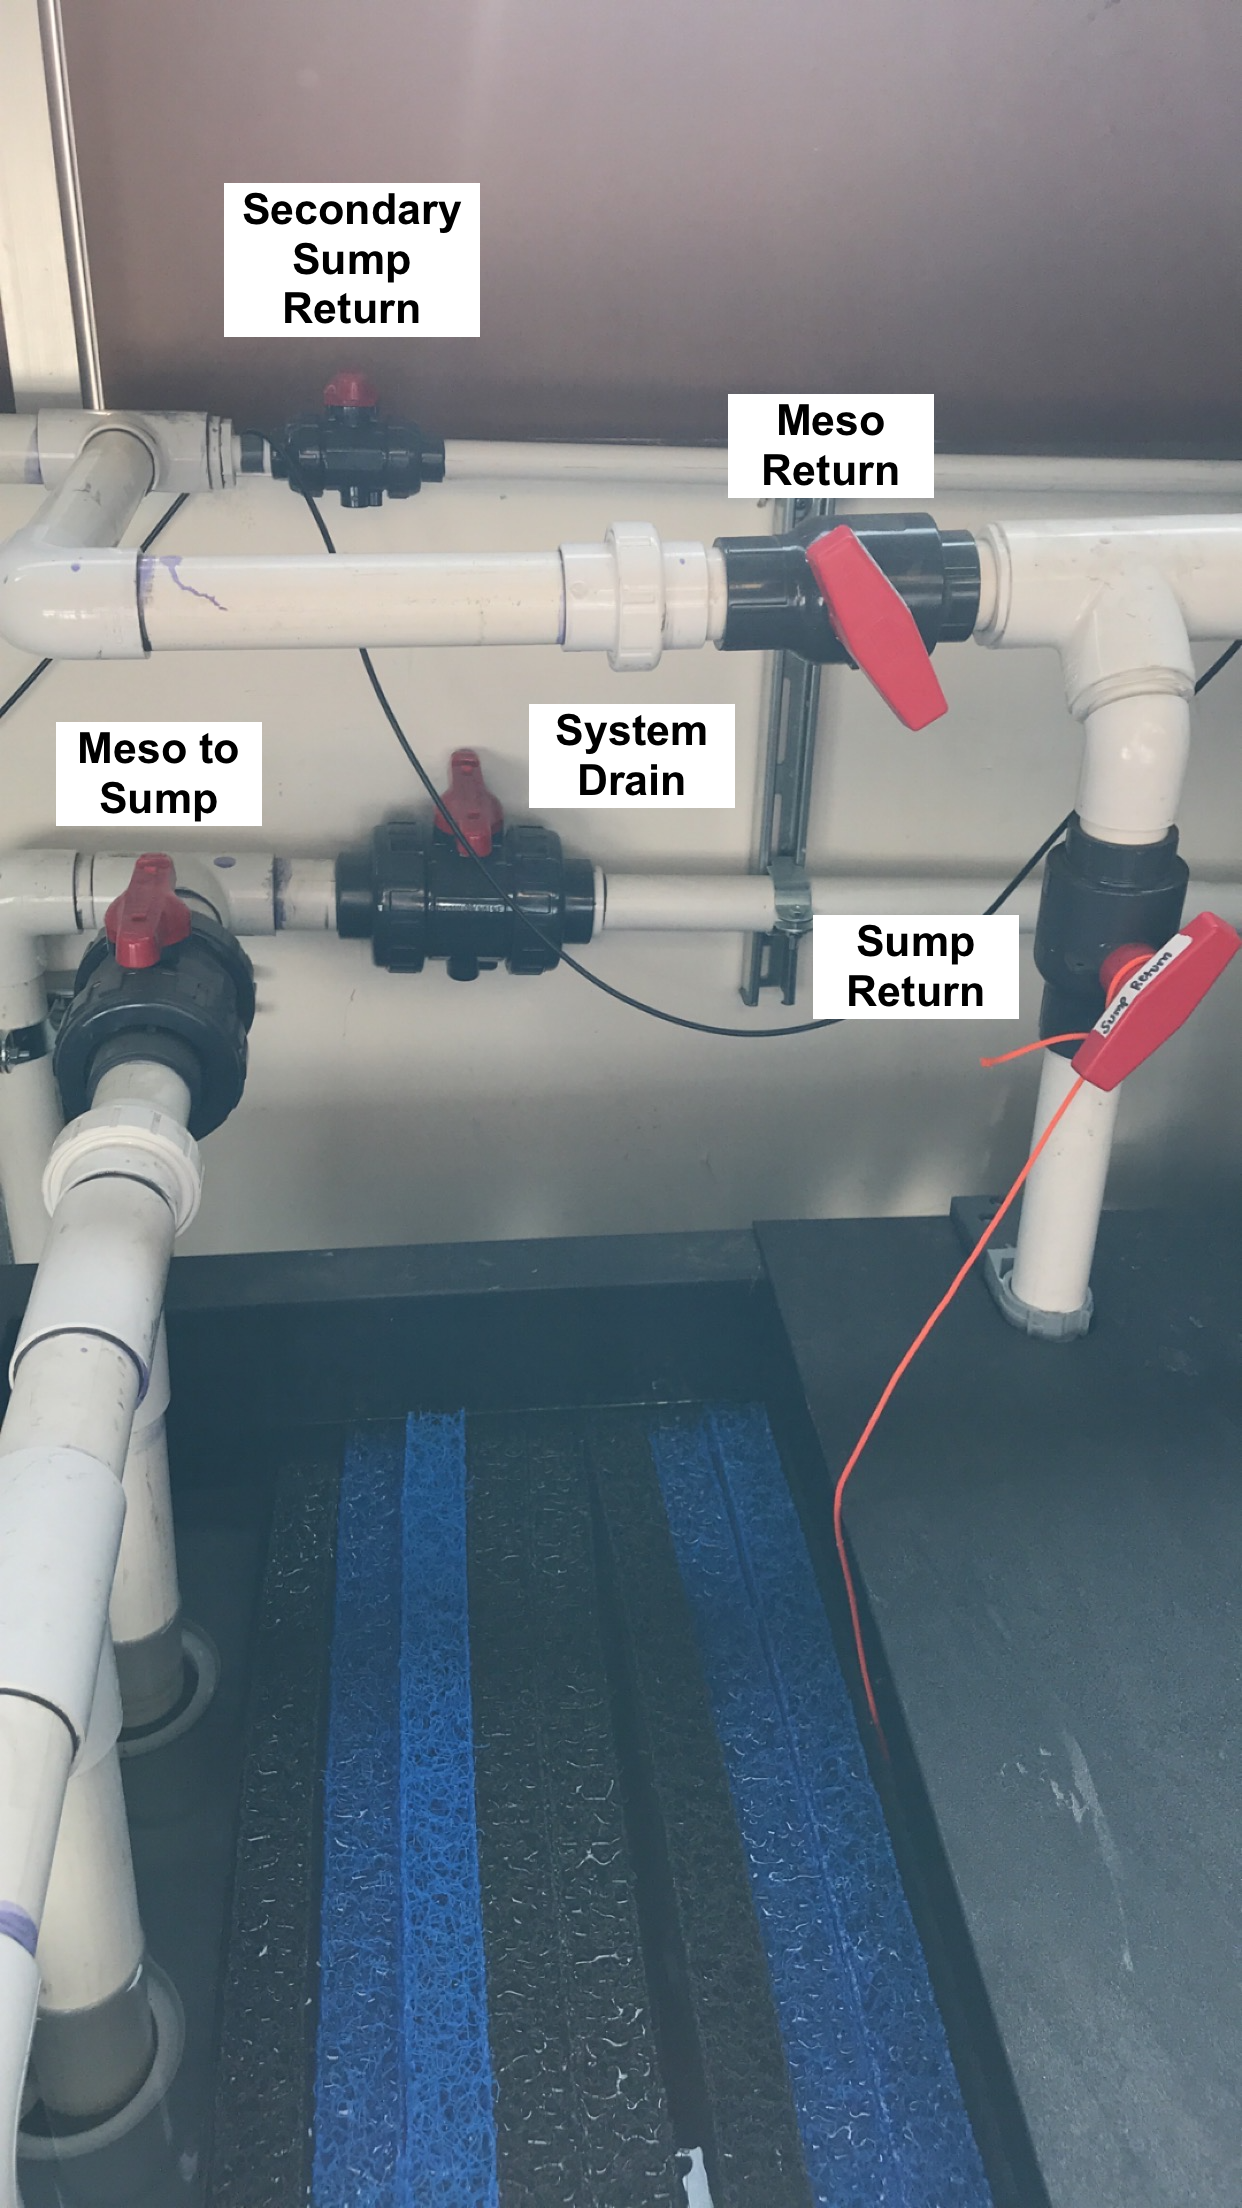
\includegraphics{images/Sump_Flow_Valves.png}\\
    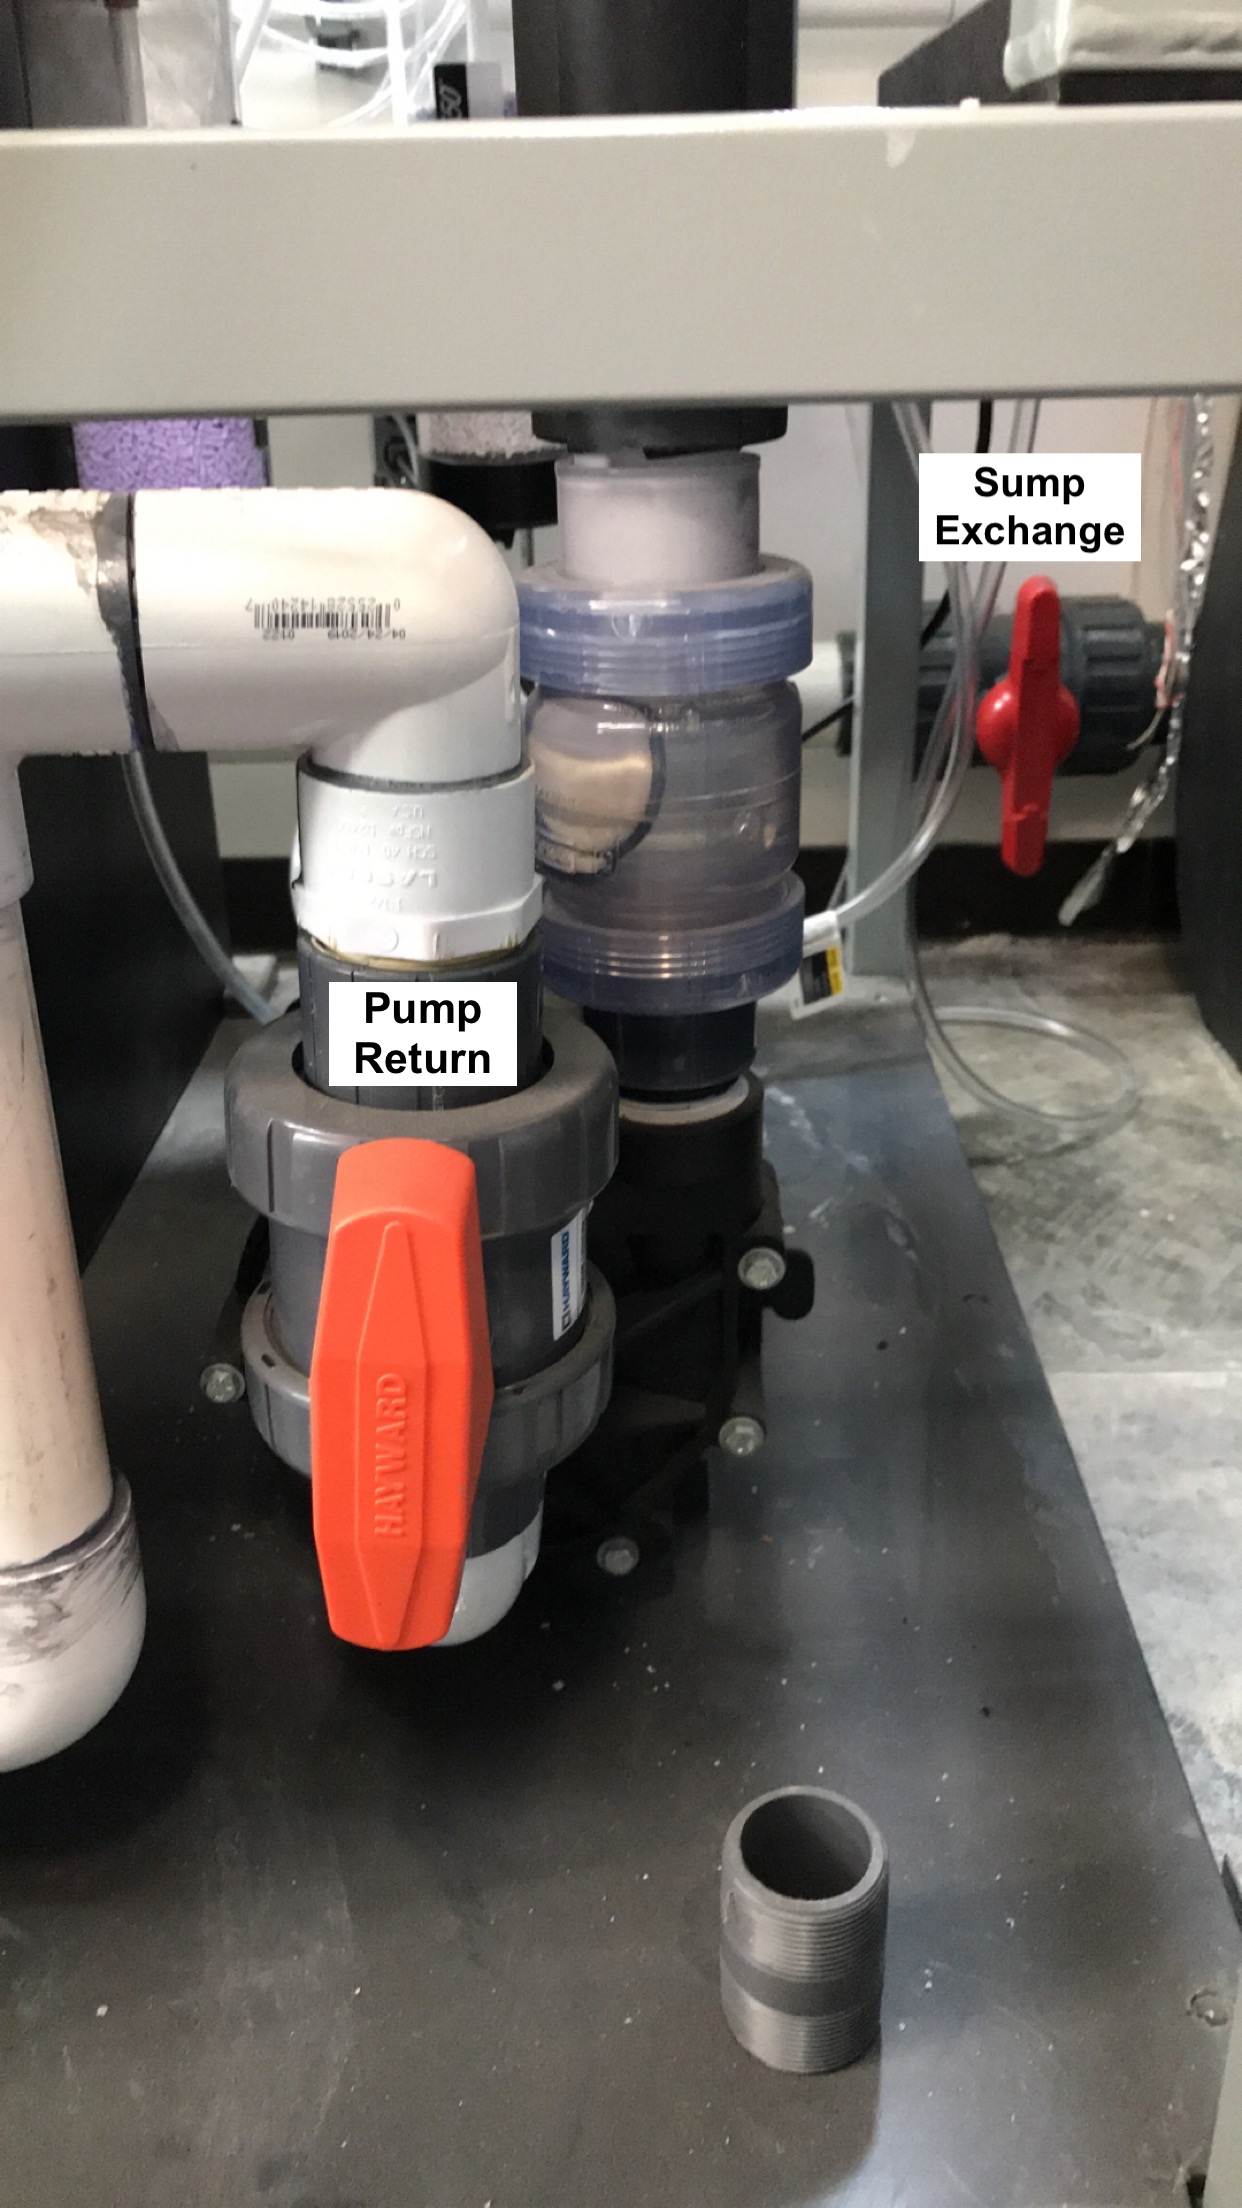
\includegraphics{images/Pump_Valve.png}\\
    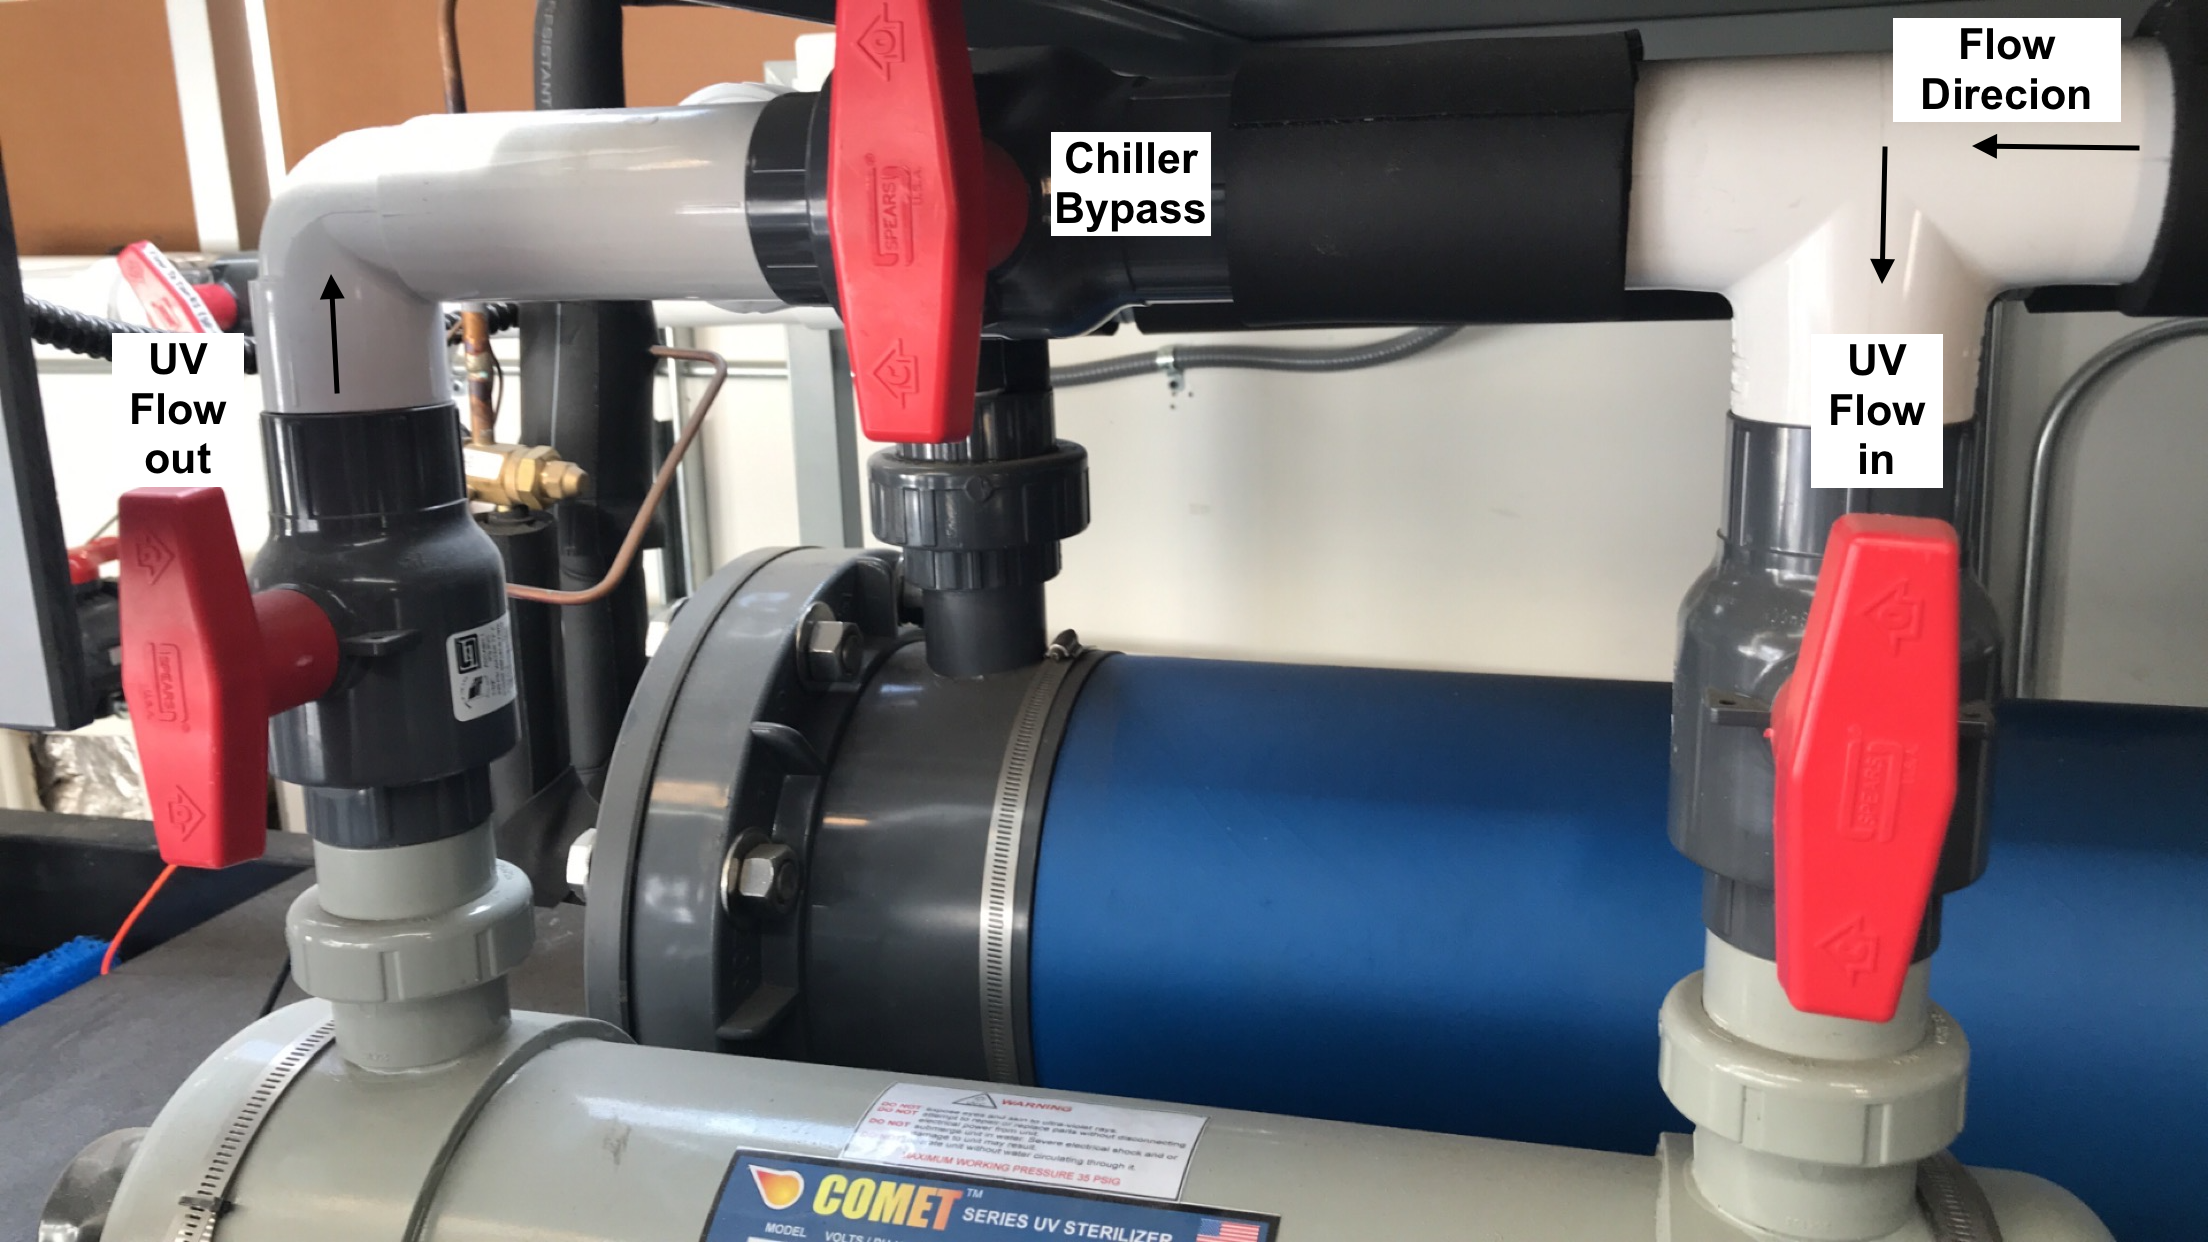
\includegraphics{images/UV_Valves.png}\\
  \end{enumerate}
\item
  Turning on sump flow

  \begin{enumerate}
  \def\labelenumii{\arabic{enumii}.}
  \tightlist
  \item
    Once all the valves are properly opened/closed as described above, plug in the Cascade Pump and make sure water is running through the system properly without any leaks. There may be some initial sputtering while air is pumped out of the pipes, but that should stop within a couple minutes.
  \item
    Look at the pump and make sure you can see water being pushed through the clear junction.

    \begin{enumerate}
    \def\labelenumiii{\arabic{enumiii}.}
    \tightlist
    \item
      If it looks like water is not running through the pump, \textbf{unplug the pump immediately}. Running the pump dry can burn out the motor.
    \end{enumerate}
  \item
    If everything seems to be stable, plug in the UV light.
  \item
    To stabilize the pH in the system, fill the PhosBan Reactors with CO2 absorption media and plug in the air pumps as \protect\hyperlink{CO2_Scrubber}{detailed below}.
  \end{enumerate}
\end{enumerate}

\textbf{Mesocosm Tank Flow}

\begin{enumerate}
\def\labelenumi{\arabic{enumi}.}
\tightlist
\item
  Filling the mesocosm tanks

  \begin{enumerate}
  \def\labelenumii{\arabic{enumii}.}
  \tightlist
  \item
    Make sure the drain valve located under each tank is closed (turned clockwise all the way, finger-tight).
  \item
    Fill each rack one at a time (only open the N flow valves for one set of 4 tanks at a time) and make sure rack and filtration skid flows are balanced before moving on to the next rack.

    \begin{enumerate}
    \def\labelenumiii{\arabic{enumiii}.}
    \tightlist
    \item
      Open the N flow valve for each tank (and S flow valve if you plan to turn on the solenoid {[}SOL-TNK-\#{]} to help fill the tanks).
    \end{enumerate}
  \item
    To open flow from the sump to the tanks, first make sure the circular flow within the sump itself is stable. Then slowly open the Meso Return valve (turn counterclockwise) until the t-valve is sitting about 45 degrees to the PVC pipe. This configuration splits flow to both the sump and the mesocosm. You can further adjust water pressure to the tanks by slightly closing the Sump Return valve to direct more flow to the meso, less flow to the sump, while always keeping the line to the sump partially open.
  \item
    Once all tanks are filled, make sure the whole system is stable in standard recirculation mode before setting up a tidal cycle, if desired.
  \end{enumerate}
\item
  Set flow in tanks

  \begin{enumerate}
  \def\labelenumii{\arabic{enumii}.}
  \tightlist
  \item
    Calculate your desired residence time. When full, each tank holds 55 liters, so divide 55L by your desired residence time and use that estimated value as your flow rate. Example: for a RT of 4 hours: 55L/4hr = 13.75 L/hr
  \item
    Use the Neptune Systems flow meters as a guide for setting the flow, but for the most accurate flow rates, use a graduated cylinder to estimate flow into each tank.

    \begin{enumerate}
    \def\labelenumiii{\arabic{enumiii}.}
    \tightlist
    \item
      Using the example above: 13.75 L/hr = 229.2 mL/min = 38.2 mL/10 seconds to efficiently check each tank's flow using a graduated cylinder
    \end{enumerate}
  \item
    While higher flow is more stable, lower flow may change slightly throughout the day, so it is recommended to check and set flow twice per day: once in the morning and once in the afternoon/evening.
  \end{enumerate}
\end{enumerate}

\textbf{CO2 Scrubber to Elevate pH}

\begin{enumerate}
\def\labelenumi{\arabic{enumi}.}
\tightlist
\item
  Filling/Replacing media in the Phosban Reactor

  \begin{enumerate}
  \def\labelenumii{\arabic{enumii}.}
  \tightlist
  \item
    Unplug the airpump connected to the Phosban Reactor and disconnect both sets of tubing going into/out of the Reactor to easily handle it.
  \item
    Unscrew the lid of the Reactor, take off the red cap and black mesh, and pour out the used up media (purple if freshly used, grayish white if used and stale) into a bag or some other containment. Used media can be deposited in a standard trash receptacle.
  \item
    Use tape or parafilm to cover the hole of the small tube inside the Reactor before pouring in the new media (stark white pellets). Fill to \textbf{an inch below} the top of the small tube, so no media falls into the tube. Remove the covering from the small tube and replace the black mesh and red cap, aligning the red cap so it encapsulates the top of the small tube.
  \item
    Screw the lid back on, finger tight, and replace the Reactor on the side of the sump. Reconnect the tubing from the airpump to the side of the Reactor and from the air splitter to the front of the Reactor. Submerge the airstones connected to the air splitter tubing in the holding reservoir of the sump.
  \item
    Once you're sure everything's securely placed, plug in the air pump.
  \item
    Listen and feel for any air leaks and adjust tubing as necessary.
  \end{enumerate}
\end{enumerate}

\textbf{Daily Checks of Sump and Tank Operation}

While the system is powered on and cycling water through the sump and mesocosm tanks, there are certain operations and parameters that should be checked for daily. This is a basic list of items that should be assessed, although you may need to incorporate additional items depending on your experimental design.
1. Is sump level normal (2 inches above white carbon filters)?
- If no, immediately unplug the Cascade pump and UV light to avoid damage
- Troubleshooting:
- Is the outside sump pump functioning? Did water overflow out of the hole?
- Are any of the mesocosm tanks overflowing?
1. Is there any overflow of water from the mesocosm tanks?
- If yes:
- Check outflow pipe blockage
- If water is being siphoned from any tanks via the tubing and lid holder, wipe off tank edges (particularly undernear the black holders) to dry off and stop the siphoning action
1. Is there adequate flow to tanks (visual check)?
- Lift up each tube enough to make sure there is relatively decent flow (for your needs) in each tank
- If no, is there inadequate flow in one tank or all tanks?
- One tank: need to increase flow via needle valve
- All tanks: may need to increase flow to mesocosm from the sump
- Using a stopwatch and graduated cylinder, measure flow rate from each tube and adjust as necessary using the needle valve above each tube
1. Is the dehumidifier full?
- The dehumidifier tray should be emptied every day to avoid humidity buildup and condensation on electronics
1. Are the tank parameters within range?
- Using handheld probes for temperature, salinity, and pH, each tank should be checked for parameter values (log these values)
- If values read by the handheld probes do not match values read by the apex (see the Apex Fusion Guide), recalibrate the incorrect probes
- If handheld probes and apex are both showing values outside of your desired range, check the apex programming (see Apex Programming Guide and Apex Fusion Guide)
- Adjust programming as necessary
- If programming is correct, check if instruments have failed
- Temperature: check heater fail or poor plug connection
- pH: check if air stones (aka bubblers) are dosing or `leaking' CO2. May need to adjust pressure on the CO2 tank to avoid CO2 pressure in tubing forcing CO2 through the solenoids if pH is too low
- Salinity: may need to schedule a water collection day to refresh the system water if salinity values are too high

\textbf{Draining the Mesocosm and Sump}

\begin{enumerate}
\def\labelenumi{\arabic{enumi}.}
\tightlist
\item
  The first step before draining any water is to turn off the powerheads, heaters, and CO2 solenoids in all mesocosm tanks. \textbf{The powerheads and heaters cannot be ON when dry or they may be damaged}.
\item
  You must also place caps on each pH probe filled with either DI water for temporary storage or KCl storage solution for long-term storage. \textbf{The probe tips cannot dry out or they will be damaged}.

  \begin{enumerate}
  \def\labelenumii{\arabic{enumii}.}
  \tightlist
  \item
    Remove the probe from its holder in the tank, rinse in DI, then carefully slide the DI-filled cap on the probe tip until the diode is fully submerged.
  \end{enumerate}
\item
  Divert flow from the mesocosm tanks to the drainage port

  \begin{enumerate}
  \def\labelenumii{\arabic{enumii}.}
  \tightlist
  \item
    There is a drain in the Mechanical Room behind the Field Room with PVC pipe facing downward inside. This PVC is connected to our system and is the location for all system drainage.
  \item
    Refer to \protect\hyperlink{Figure1}{Figure 1} for the following t-valve identities.
  \item
    \textbf{First open the System Drain Valve} by turning the valve so it aligns parallel to the PVC. This opens flow to the drainage port in the back room. Always open an avenue of flow before closing an avenue of flow to avoid back pressure build up.
  \item
    Second, Close the Meso To Sump valve by turning the valve so it sits perpendicular to the PVC. This will divert flow from the mesocosm tanks out of the system.
  \end{enumerate}
\item
  Fully open (parallel to the PVC) the Sump Return valve of the filtration system, then turn off the flow of both the N and S valves for each tank, turning the valves clockwise until finger tight.
\item
  Unplug the UV light and air pumps, but leave the water pump on for now.
\item
  When draining the tanks, drain one tank at a time, to not overflow the drainage system.

  \begin{enumerate}
  \def\labelenumii{\arabic{enumii}.}
  \tightlist
  \item
    \textbf{Unscrew} the larger outflow pipe until it is fully removed and cover the top opening with your hand to avoid water splashing upward when you remove the pipe.
  \item
    Under each tank is a needle valve controlling drain flow through the smaller outflow pipe in each tank. Fully open this valve by turning the needle counterclockwise until partially open.
  \item
    The smaller outflow tube can simply be pulled out from its slot, sometimes needing to be twisted to be unwedged.
  \end{enumerate}
\item
  The underground sump pump located between the Mesocosm container and the Field Room will continue to push water from the tanks to the Field Room system.

  \begin{enumerate}
  \def\labelenumii{\arabic{enumii}.}
  \tightlist
  \item
    \textbf{Do not allow salt water to overflow the drainage port of the Mechanics room.} Periodically check the drainage port to make sure the water pumped from the tanks is not overflowing onto the floor of the Mechanical Room.
  \item
    By only draining one tank at a time, overflow should not be an issue.
  \item
    If you notice water is overflowing, slightly open the Meso To Sump valve to divert some water back into the sump and reduce the water volume diverted to the drainage port.
  \end{enumerate}
\item
  Once the mesocosm tanks are all drained, unplug the sump's main pump.

  \begin{enumerate}
  \def\labelenumii{\arabic{enumii}.}
  \tightlist
  \item
    \textbf{Alternatively}, to drain the sump partially, leave the main pump plugged in, open the N flow valves for mesocosm tanks, then slightly open the Meso Return valve, and slightly close the Sump Return Valve.
  \item
    Water will flow from the sump to the tanks, then out through the drainage port.
  \item
    Once the water level in the sump is 1-2 inches above the three carbon filters, open the Return Sump valve, then close the Meso Return valve, then unplug the sump's main pump.
  \end{enumerate}
\item
  Remove filters from the sump

  \begin{enumerate}
  \def\labelenumii{\arabic{enumii}.}
  \tightlist
  \item
    To access the bio-filtration reservoir, remove the black and blue matala mesh filters, and clean them by hosing them down with freshwater (available just outside the Field Room door).
  \item
    To remove the 50-micron mesh filters, remove the PVC pipe located directly after the Meso To Sump valve (see \protect\hyperlink{Figure1}{Figure 1}) by unscrewing the PVC at the junction (unscrew away from you if standing at the head of the sump). This PVC pipe with three outports can be temporarily removed, so the mesh can be taken out and also sprayed down with fresh water to clean.
  \item
    Remove the three carbon filters from the main reservoir by gently twisting and tugging until they come away, and hose them down outside with fresh water.
  \end{enumerate}
\item
  To drain the sump, use a small aquarium pump to pull water out of the sump into buckets that can be drumped down the drainage port in the back room

  \begin{enumerate}
  \def\labelenumii{\arabic{enumii}.}
  \tightlist
  \item
    Attach tubing to the aquarium pump and place both the pump and tubing end into the main reservoir of the sump.
  \item
    Plug the aquarium pump into the quad outlet behind the sump (where the sump pump and UV light had previoiusly been plugged in).
  \item
    Use the tubing to fill up a bucket with remaining sump water, and place the tubing end back into the sump when dumping the bucket.
  \item
    Do this until the water level is such that the aquarium pump is no longer a viable option. 1. \textbf{Do not let this pump run dry, or it may be damaged}
  \end{enumerate}
\item
  Place the tubing and aquarium pump in the bio-filtration reservoir and continue the process, stopping before the pump runs dry.

  \begin{enumerate}
  \def\labelenumii{\arabic{enumii}.}
  \tightlist
  \item
    Any additional water can be removed with a small bucket or large sponge.
  \end{enumerate}
\item
  Once the system is drained of seawater, place the filters back into the sump (3 50um mesh, 8 bio-filters, and 3 carbon filters).
\item
  Clean the mesocosm tanks thoroughly.

  \begin{enumerate}
  \def\labelenumii{\arabic{enumii}.}
  \tightlist
  \item
    Remove any debris or algal grwoth
  \item
    Wipe off all probes (avoiding sensitive tips), tubes, heaters, and sides of the tanks
  \item
    Use a brush to clean inside the large and small outflow pipes
  \item
    Thoroughly clean the powerheads (remove the plastic head and magnetic turbnine within to clean all areas of each unit, removing algal growth and debris)
  \end{enumerate}
\item
  Screw back on the PVC pipe with three outports at the junction by the Meso To Sump valve.
\item
  Fill the sump with fresh water.

  \begin{enumerate}
  \def\labelenumii{\arabic{enumii}.}
  \tightlist
  \item
    Follow the instructions in the \href{06-water_collection.md}{Water Collection Guide for filling the sump} with fresh water (attach a hose to the water pipe next to the Field Room door and fill the sump from the hose) and the order of operations for turning flow back on through the sump and tanks.
  \item
    You will not have to plug in the UV light or air pumps since you are not maintaining any water chemistry, but rather just flushing the system.
  \item
    Place the hose in the front most compartment of the sump (where the three 50um mesh filters sit, to let the fresh water go through this compartment, into the second compartment and then overflowing into the main reservoir.
  \item
    While the sump main reservoir fills to about halfway, open the N and S flow valves for all the tanks.
  \item
    Once the sump is halfway full, partially open the Meso Return valve and partially close the Return to Sump valve.
  \item
    Plug in the sump main pump.

    \begin{enumerate}
    \def\labelenumiii{\arabic{enumiii}.}
    \tightlist
    \item
      Fresh water from the sump will flow through the sump pipes and into the mesocosm, flushing out the internal plumbing, and then from the tanks, into the underground sump, and out through the drainage port. Flush the system in this way for \textasciitilde{} 20 minutes, leaving the hose on to continuously refill the sump.
    \item
      Make sure the sump is not filling up too quickly (avoid overflowing) or draining too quickly (avoid the water level dropping below 1-2 inches above the three carbon filters)
    \end{enumerate}
  \item
    After the system has flushed through, re-place each mesocosm tank's outflow pipes (screw in the large pipes and wedge in the small pipes), and then close the D valve below each tank.
  \item
    Open the Meso to Sump valve and close the System Drain valve.
  \item
    Allow all tanks to completely fill with fresh water, and once the tanks are full and the sump is filled halfway, turn off and remove the freshwater hose.
  \end{enumerate}
\item
  Let fresh water run through the system for one to two days before following these same steps for draining the freshwater.
\item
  End of experiment

  \begin{enumerate}
  \def\labelenumii{\arabic{enumii}.}
  \tightlist
  \item
    Remove the water inflow tubes from each tank's N and S ports to be acid washed and rinsed in DI water before next use.
  \item
    Rinse all pH, conductivity, and temperature probes in DI water.
  \item
    Use a KCl storage solution for capping the pH probes, ensuring the probe tips are fully submerged in the solution.
  \end{enumerate}
\end{enumerate}

\textbf{Overflow into Secondary Sump}

\begin{enumerate}
\def\labelenumi{\arabic{enumi}.}
\tightlist
\item
  If you need to contain more water in the system than the tanks and main reservoir can hold at one time (ex. during a ``low tide event'' when half of the tank water is drained into the sump), then you will need to incorporate flow to and from the secondary sump.
\item
  First unplug the sump's main water pump to make sure the pump will not run dry if the water level drops too low (see details below).
\item
  To direct some flow from the mesocosm system into the secondary sump, partially or fully open the Secondary Sump Return valve ( \protect\hyperlink{Figure1}{Figure 1} ), so that the t-valve runs parallel with the PVC. Filtered sump water will then be simultaniously directed into the mesocosm and the secondary sump, via PVC tubing that diverts water into the top of the secondary reservoir.
\item
  To then open flow between both the main holding reservoir and the secondary sump, open the Sump Exchange valve ( \protect\hyperlink{Figure2}{Figure 2} ), so the t-valve runs parallel with the PVC.

  \begin{enumerate}
  \def\labelenumii{\arabic{enumii}.}
  \tightlist
  \item
    Because this flow-through connection will allow water to flow between both reservoirs to establish water level equilibrium, make sure the water level in the main reservoir is still about 2 inches above the carbon filters after this water exchange has occurred. If not, add more seawater to the system until the carbon filters are once again submerged \textbf{to avoid the pump running dry}.
  \item
    Once the carbon filters are appropriately submerged (seawater just two inches above the filters, not much more), turn the main pump back on.
  \item
    The full system requires \textasciitilde{} 400 gallons of sea water to maintain tank volume and submersion of carbon filters while including use of the secondary sump.
  \end{enumerate}
\end{enumerate}

\hypertarget{water-collection-procedures}{%
\chapter{Water Collection Procedures}\label{water-collection-procedures}}

The water collected for the mesocosm system is filtered (100um mesh filter) unbuffered seawater from the Southern California Marine Institute (SCMI) located at 820 S Seaside Ave, San Pedro, CA 90731.

\textbf{Contents}\\
- \protect\hyperlink{packing_list}{\textbf{SCMI Packing List}}\\
- \protect\hyperlink{check_list}{\textbf{Pre-Collection Check List}}\\
- \protect\hyperlink{water_flow}{\textbf{Water Flow Procedure}}\\
- \protect\hyperlink{water_collection}{\textbf{Water Collection}}\\
- \protect\hyperlink{filling_the_sump}{\textbf{Filling the Sump}}

\textbf{SCMI Packing List}

\begin{enumerate}
\def\labelenumi{\arabic{enumi}.}
\tightlist
\item
  Items to bring to SCMI for collecting water

  \begin{enumerate}
  \def\labelenumii{\arabic{enumii}.}
  \tightlist
  \item
    Two large water storage bins and lids
  \item
    Pool hose (stored inside one of the water bins)
  \item
    Standard garden hose (from Field Room)
  \item
    Triple filter and locking ring
  \item
    Banjo attachment (PVC to pool hose adaptor)
  \item
    Two ratchet straps or sets of rope
  \end{enumerate}
\end{enumerate}

\textbf{Pre-Collection Check List}

\begin{enumerate}
\def\labelenumi{\arabic{enumi}.}
\item
  Before traveling

  \begin{enumerate}
  \def\labelenumii{\arabic{enumii}.}
  \tightlist
  \item
    Sign out the Ford 450 truck at the Bio Stock Room for your desired day (Biology Department Vehicle ID 440).

    \begin{enumerate}
    \def\labelenumiii{\arabic{enumiii}.}
    \tightlist
    \item
      Before driving a univeristy vehicle, be sure to complete the Defensive Drivers course. Email Wendy Dunbarr (\href{mailto:wendy.dunbarr@csun.edu}{\nolinkurl{wendy.dunbarr@csun.edu}}) for details.
    \end{enumerate}
  \item
    At least 24 hours before collecting water, email Mark Loos (\href{mailto:mark.loos@csulb.edu}{\nolinkurl{mark.loos@csulb.edu}}) of your intent to get water, and give him an estimated time of arrival. Check in with him or his appointed staff member upon arrival.
  \item
    Check that all three o-rings of the triple filter are in place and that the filters are placed in order (left to right following direction of flow: 20um, 5um, 1um) before twisting the filters onto the base rack. Use the locking ring to ensure a tight seal of the filter compartments onto the rack.
  \item
    Ensure that all components of the sump are prepared for water:

    \begin{enumerate}
    \def\labelenumiii{\arabic{enumiii}.}
    \tightlist
    \item
      Three bag filters are in place
    \item
      Eight matala filters are in place
    \item
      Three carbon filters are in place, the open PVC end wedged into the holes of the PVC located in the back of the holding tank
    \item
      If you do not intend to use the secondary sump, close the Sump Exchange valve (see image below)
    \item
      Check that all power cords are away from areas with possible water exposure
    \end{enumerate}
  \end{enumerate}

  \begin{figure}
  \centering
  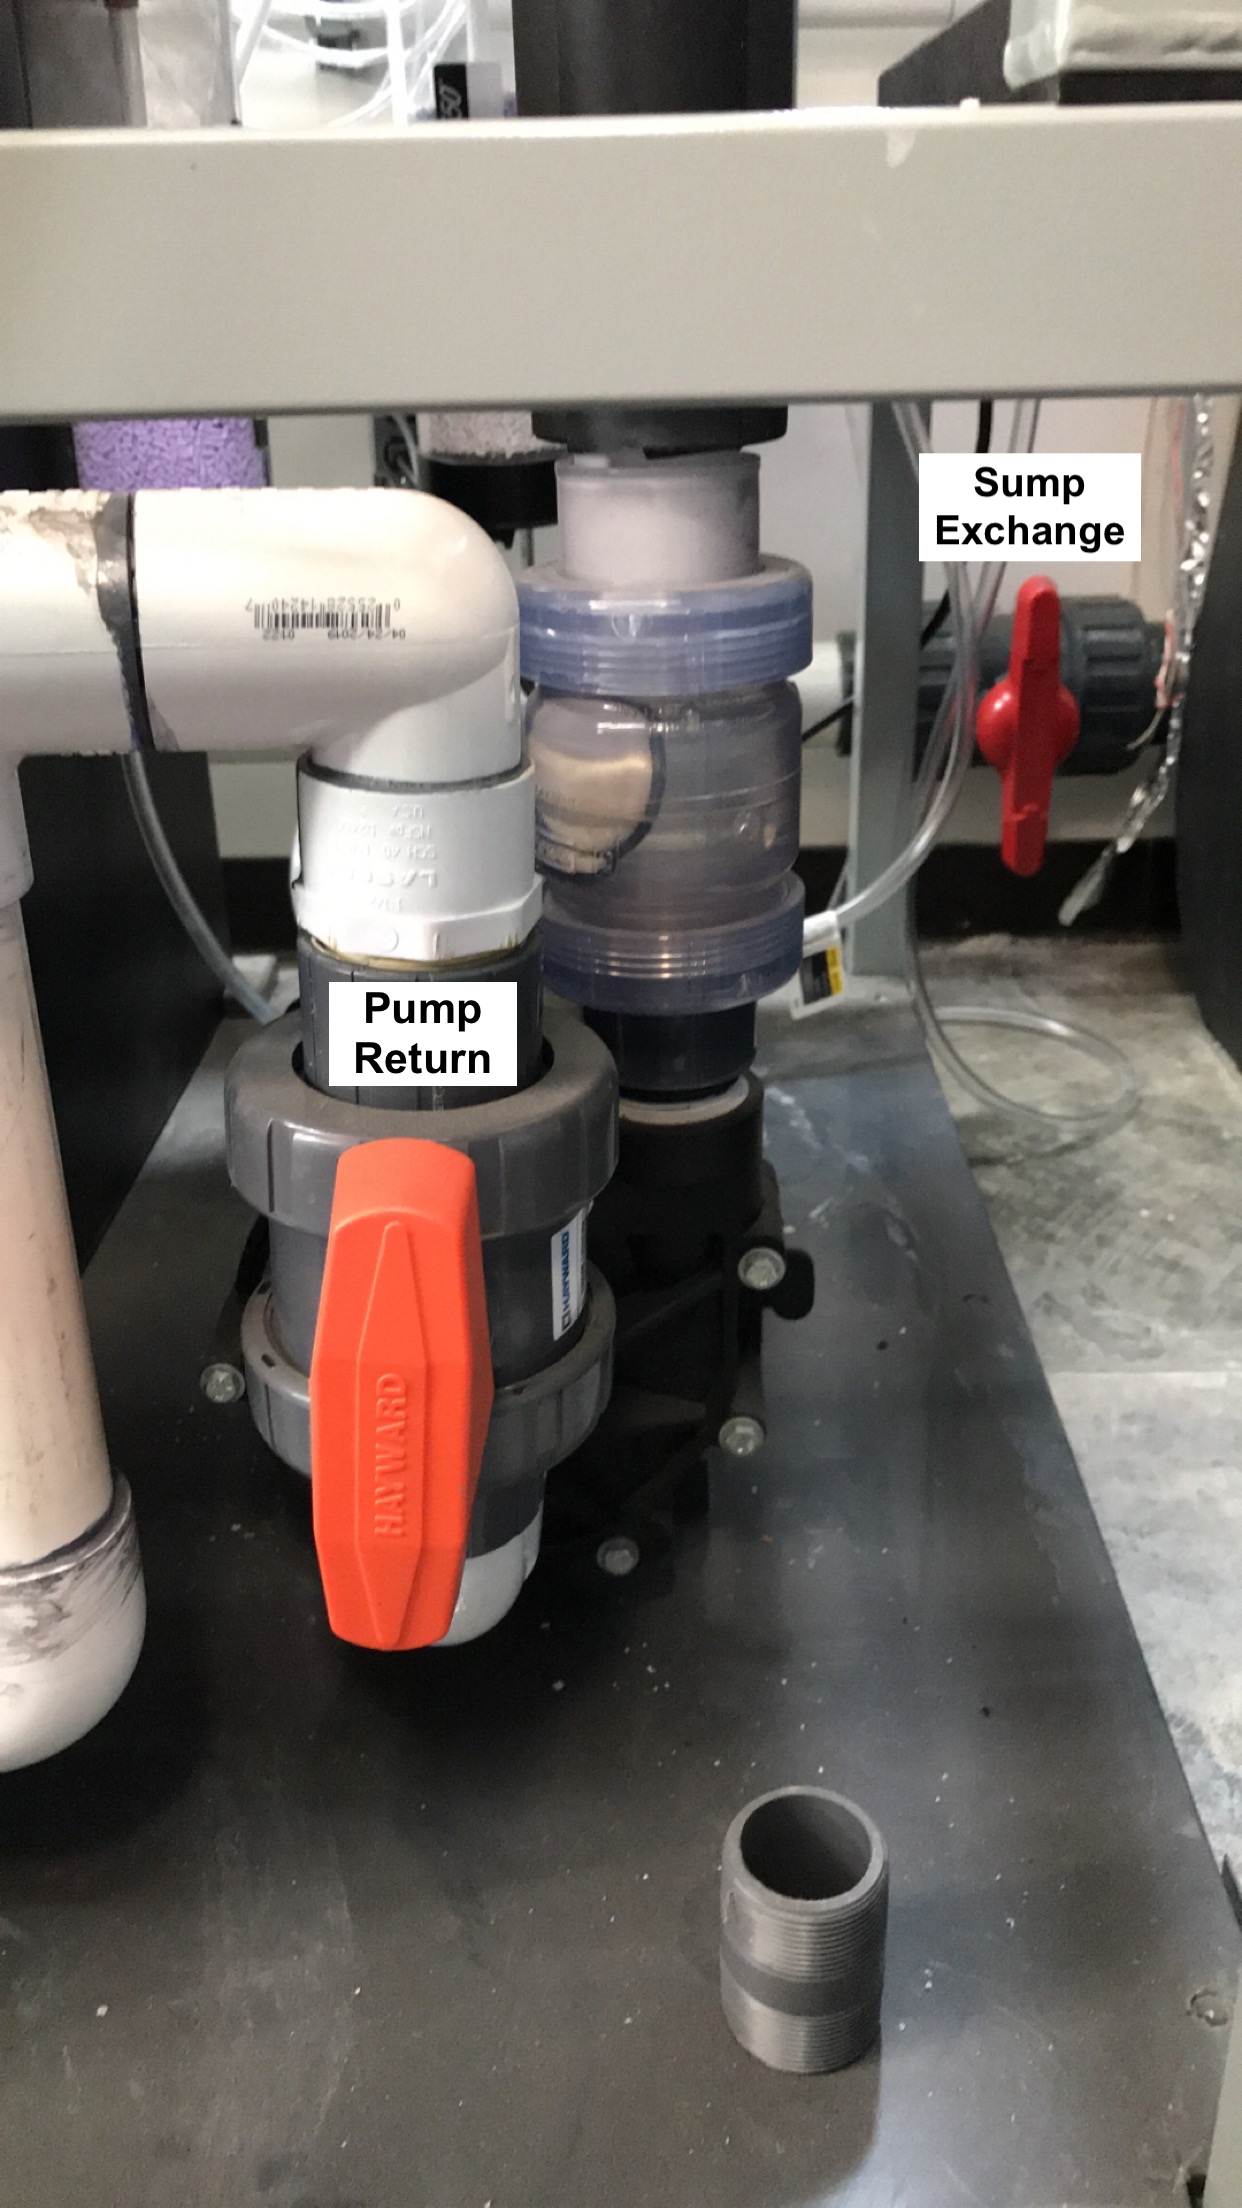
\includegraphics{images/Pump_Valve.png}
  \caption{Figure 1. Sump Exchange valve}
  \end{figure}
\item
  Once you pick up the truck from behind Chaparral Hall, back it up to the large stacked square bins in the same parking lot, near the side of the building on the grass.

  \begin{enumerate}
  \def\labelenumii{\arabic{enumii}.}
  \tightlist
  \item
    With the help of at least one other person, lift and slide the top bin into the bed of the truck. Take off the lid of the second bin and lift the second bin onto the bed of the truck. Once in place, put the lid back on (lids weight an additional 15-20lbs).
  \end{enumerate}
\item
  Make sure you have all the items listed above laoded in the truck to bring to SCMI.
\item
  Plan to leave CSUN for SCMI after 9am to avoid major traffic, and wear or bring closed toed shoes to wear once you arrive.
\item
  When you arrive at SCMI, back into the employee lot (the parking lot to the left of the building when looking on from the street), back through the lot and behind the building parallel to the wire fence.

  \begin{enumerate}
  \def\labelenumii{\arabic{enumii}.}
  \tightlist
  \item
    Move the cone before backing into the lot behind the building and replace the cone when you leave.
  \end{enumerate}
\end{enumerate}

\textbf{Water Flow Procedure}

\begin{enumerate}
\def\labelenumi{\arabic{enumi}.}
\item
  Near the wire fence, there is a large pool hose with a pvc loop attachment. Remove the banjo attachemnt comprising of the PVC ``U'' on the pool hose and attach the banjo adapter that connects to the triple filter. Before connecting it to the filter, move this end of the hose to the drain port (hole in the concrete flowing under the walkway).
\item
  Unwind the SCMI garden hose enough to also place the outflow end at the drain port.
\item
  Open the t-valve at the base of the pool hose \textbf{half-way (at a 45 degree angle)} and fully open adjacent garden hose (t-valve parallel to the PVC).

  \begin{enumerate}
  \def\labelenumii{\arabic{enumii}.}
  \tightlist
  \item
    Refernce image for t-valve alignment:
  \end{enumerate}

  \begin{figure}
  \centering
  \includegraphics{images/SCMI_hose_valves.png}
  \caption{Figure 2. Hose T-valve Alignments}
  \end{figure}
\item
  Walk over to the filtration area in the corner of the back lot (near the fish pens) and locate the filter chamber (tall teal cylinder with rounded top). Open the t-valve for the PVC pipe running from the base of the filter chamber toward the wire fence (see image below).
\item
  There is a power switch on the fence across from the filter's PVC (second power unit from the right). Turning this switch ON will initiate flow from the marina, through the filter, and out the end of the pool hose.

  \begin{enumerate}
  \def\labelenumii{\arabic{enumii}.}
  \tightlist
  \item
    \textbf{Do not turn on the power supply until you have opened the other t-valves.} Doing so could cause pressure buildup in the piping and damage the system.
  \end{enumerate}
\item
  Flip the switch ON and leave the water running for 30 seconds to 1 minute to flush out any standing water in the system.

  \begin{figure}
  \centering
  \includegraphics{images/SCMI_filter_pvc.png}
  \caption{Figure 3. SCMI Filter System}
  \end{figure}
\end{enumerate}

\textbf{Water Collection}

\begin{enumerate}
\def\labelenumi{\arabic{enumi}.}
\item
  Connect the male end of the garden hose to the outflow end of the triple filter, and place the female end inside one of the bins (you will need to remove or offset the bin lids).
\item
  When you have finished flushing out the system and are ready to fill the bins, turn off the power supply without closing off any of the t-valves.
\item
  Attach the banjo adapter to the triple filter (see image below), then turn on the power supply again. This will initiate flow through the filters and into the bins. To avoid pressure build-up in the system, allow the SCMI garden hose to continuously pump water into the drain port.

  \begin{figure}
  \centering
  \includegraphics{images/Triple_filter.png}
  \caption{Figure 4. Triple Filter}
  \end{figure}
\item
  Filling the bins

  \begin{enumerate}
  \def\labelenumii{\arabic{enumii}.}
  \tightlist
  \item
    If you are filling up the entire mesocosm system, you will need to fill both bins about 3/4 full twice to obtain 400 gallons, requiring two trips to SCMI.
  \item
    If you are only doing a partial water change or refill, fill the bins with slightly more than you need in case any water is lost en route to CSUN.
  \end{enumerate}
\item
  When you are finished filling, \textbf{first turn off the power supply}, then close the t-valve on the pipe between the power supply and the filter chamber, and finally close the t-valves at the base of the hoses.

  \begin{enumerate}
  \def\labelenumii{\arabic{enumii}.}
  \tightlist
  \item
    CLosing off any t-valves before shutting off the power could cause a pressure build-up in the PVC and may rupture the system.
  \end{enumerate}
\item
  Place the lids on the water containers and use the ratchet straps or rope to secure the bin lids down (this will help with water spillage on the drive back to CSUN).
\item
  Remove the banjo adapter from the pool hose and the triple filter, and replace the PVC ``U'' back on the pool hose.
\item
  Remove the garden hose from the triple filter, then tilt the triple filter upside down to allow water inside the filter chambers to flow out before loading it back in the truck.
\end{enumerate}

\textbf{Filling the Sump}

\begin{enumerate}
\def\labelenumi{\arabic{enumi}.}
\tightlist
\item
  Once back at CSUN, pull into the laoding bay between Citrus and Eucalyptus, and back up to the Field Room, leaving just enough space to open the door.
\item
  Unstrap and remove the lids. Place one end of the large pool hose in one of the containers, and use a weight to keep it from floating up.
\item
  Pull the free end of the hose to the sump, and start a siphon. Gently wedge the end of the hose in between the matalamesh filters in the sump for hands-free siphoning and to filter the water as it goes into the system.

  \begin{enumerate}
  \def\labelenumii{\arabic{enumii}.}
  \tightlist
  \item
    To start a gravity-fed siphon, fill the hose with as much water as you can, displacing the air. Keep one end of the hose weighed down in the seawater container and the other end wedged in the sump. Starting near the sump end of the hose and working toward the bin end, lift the hose section by section to redirect the bulk of the water within toward the bin end until at least 1/3 of the hose at the bin end is filled with water. Lower the hose section you are holding to return flow back toward the sump end.
  \end{enumerate}
\item
  When water volumne in the first bin is nearly at the top of the hose opening, remove the weight while holding down the hose opening toward the bottom of the bin.

  \begin{enumerate}
  \def\labelenumii{\arabic{enumii}.}
  \tightlist
  \item
    Keep the opening at an angle to the bottom to allow for continued suctioning of water without exposure to air.
  \end{enumerate}
\item
  When you are ready to switch bins, preserve the siphon by cupping the palm of your hand against the hose end, submerging the hose in the next bin, then removing your hand. Place the weight again to avoid the hose floating to the surface.
\item
  If you plan to collect water again that day, simply replace the lids once you have finished siphoning, and drive back to SCMI for another round.
\item
  Once you are finished filling the sump and emptying the bins, attach the garden hose to the fresh water tap on the outside of the Field Room, and turn on water by using the metal screw key hanging on a pipe just inside the Field Room door to the left.
\item
  Hose down the entire back, bed, and sides of the truck, everything that may have been exposed to salt water. Also unscrew the filter chambers of the triple filter and hose down the chambers, the rack, and the filters sufficiently to clean off any debris or particulates.
\item
  Place the large pool hose back in one of the bins, and once you turn off the hose water, replace the key and store the garden hose back in the Field Room.
\item
  Before parking the truck, back it up to the same location where you picked up the bins, and drop/place the bins back on the grass. If there is any water left in the bins, dump that out before leaving them stacked.
\end{enumerate}

\hypertarget{tidal-manipulation}{%
\chapter{Tidal Manipulation}\label{tidal-manipulation}}

Controling the tidal cycle of each experimental tank with the Apex. This is achieved by manipulating the incoming and outgoing flow rates of each individual tank with the needle valves described in the \protect\hyperlink{system-details}{System Details}, and setting the ON/OFF time cycle of the supply line with the solenoid. The basic procedure is outlined below.

\begin{enumerate}
\def\labelenumi{\arabic{enumi}.}
\tightlist
\item
  Set the flow rate of the supply line N{[}\#{]}FLW (without the solenoid), for example 10.5 Liters/Hr, by slowly turning the black knob counterclockwise to increase flow or clockwise to decrease flow.

  \begin{enumerate}
  \def\labelenumii{\arabic{enumii}.}
  \tightlist
  \item
    You can view rates on the Fusion dashboard.
  \item
    Note that the Apex controller has some lag time in registering the flow rate after the valve has been adjusted, and the delay can be up to 30 seconds or more, so make small adjustments and monitor the change on Fusion.
  \item
    Once the rate is set you should check periodically to make sure the rate has not changed both on Fusion and by using a graduated cylinder and a timer.
  \end{enumerate}
\item
  Adjust the outgoing flow rate of the drain line D{[}\#{]}FLW higher than the N{[}\#{]}FLW, for example 15 Liters/Hr.

  \begin{enumerate}
  \def\labelenumii{\arabic{enumii}.}
  \tightlist
  \item
    With the above condition, the outgoing flow rate is higher than the incoming, so this will create a low tide effect over a 5-5.25 hr period.
  \end{enumerate}
\item
  To create a high tide effect, change the setting of SOL-TNK-\# (outlets 3 and 7 on each EB832) to ON on the Fusion dashboard, then manually turn on and adjust the flow rate of the supply line S{[}\#{]}FLW , for example 10 Liters/Hr.\\
\item
  Once the S{[}\#{]}FLW is set, change the setting of SOL-TNK-\# to AUTO on the Fusion dashboard.

  \begin{enumerate}
  \def\labelenumii{\arabic{enumii}.}
  \tightlist
  \item
    With the above condition, the total incoming flow rate (N+S) is higher thatn the outgoing (D), so this will create a high tide effect over a 5-5.25 hr period.
  \item
    For a constant ON/OFF cycle over a 12.5 hour period, the Advanced program should look like the program below:
  \end{enumerate}
\end{enumerate}

Fallback ON\\
Osc 000:00/375:00/375:00 then ON

\begin{enumerate}
\def\labelenumi{\arabic{enumi}.}
\tightlist
\item
  In the event the EnergyBar loses connection with the Apex Base, ``Fallback ON'' will keep the solenoid open, allowing water to continuously flow from S{[}\#{]}FLW.\\
\item
  The oscillate (Osc) command as written will open flow from S{[}\#{]}FLW for 6.25 hours, initiating the High Tide scenario, then close for 6.25 hours, initiating the Low Tide scenario. This will provide the effect of two high and two low tides of a semidiurnal tidal cycle over a 25 hour period.

  \begin{enumerate}
  \def\labelenumii{\arabic{enumii}.}
  \tightlist
  \item
    Using the flow rates stated above, each tidal shift will last 5.25 hours and maintain the tide height for 1 hour.
  \end{enumerate}
\end{enumerate}

For more advanced programming features, see the \href{https://github.com/SilbigerLab/Mesocosm_User_Manual/tree/7503b88686aef920c4a4ed473b1efe37b34dae10/Manuals/Apex_Comprehensive_Reference_Manual.pdf}{Comprehensive Manual}. Start on Page 65 for Seasonal Features and Moon cycles.

\hypertarget{controlling-ph}{%
\chapter{Controlling pH}\label{controlling-ph}}

The pH is controlled with the addition of CO\textsubscript{2} gas to the system. The gas is delivered to the tank by air stone and is controlled through the Apex Controls with a solenoid valve connected to the EB832.

\begin{enumerate}
\def\labelenumi{\arabic{enumi}.}
\item
  Once the CO\textsubscript{2} regulator is connected to a tank, open the main tank valve.
\item
  Use the pressure adjusting screw (larger knob in front with Tunze label) to adjust the pressure (in bar) on the pressure gauge. Turning \textbf{clockwise to open}, thus increasing pressure, while turning \textbf{counterclockwise to close}, thus reducing pressure.
\item
  The pressure should be set to 0.5 up to 1 bar on the gauge (\textasciitilde7.5psi) - ideally 0.6 bar.
\item
  Open the fine adjustment valve (smaller valve next to the tubing connecting the regulator to the tanks) to allow gas to the tank solenoid. If the pressure on the gauge is too high this may prevent the CO\textsubscript{2} solenoid from completely closing, which will inject excess CO\textsubscript{2} into the system.
\item
  Programming the solenoid for a consistent pH: pH-TNK-\#

  \begin{enumerate}
  \def\labelenumii{\arabic{enumii}.}
  \tightlist
  \item
    From your ApedFusion dashboard, click the icon for Outlets
  \item
    Find the gear icon in the upper right-hand corner of the Outlets page and select ``Add a Virtual Outlet''
  \item
    Label the outlet to be specific for the tank and treatment for a particular time block (see example below)
  \end{enumerate}

  Control type: pH Control\\
  Probe name: pH\\
  Fallback: OFF\\
  High Value: 8.2\\
  Low Value: 7.9\\
  On when: High
\item
  Programming the solenoid for diel variance:

  \begin{itemize}
  \tightlist
  \item
    Using Advanced programming and Virtual outlets
  \item
    Create a unique virtual outlet for every time block which requires a different pH, and for every tank/probe which requires that pH treatment.
  \item
    Virtual Outlet Example (for the 6 hours between 6:31am and 12:30pm, the CO2 solenoid will dose CO2 into tank 1 while the probe reads 8.10 or above):
  \end{itemize}

  Fallback OFF\\
  Set OFF\\
  If Time 06:31 to 12:30 Then ON\\
  If pH-1 \textless{} 8.10 Then OFF

  \begin{itemize}
  \tightlist
  \item
    Advanced Program Example (Every 6 hours, the pH setpoint changes, and each of the four time blocks has a unique virtual outlet name, as presented below in the four programming lines. The CO2 solenoid will dose the tank when the conditions of the virtual outlet program are met):
  \end{itemize}

  Fallback OFF\\
  Set OFF\\
  If Output pH\_1\_630 = ON Then ON\\
  If Output pH\_1\_1230 = ON Then ON\\
  If Output pH\_1\_1830 = ON Then ON\\
  If Output pH\_1\_0030 = ON Then ON
\end{enumerate}

Refer to \href{https://github.com/SilbigerLab/Mesocosm_User_Manual/tree/7503b88686aef920c4a4ed473b1efe37b34dae10/Manuals/Apex_Comprehensive_Reference_Manual.pdf}{Comprehensive Manual} for set point programming.

\hypertarget{controlling-temperature}{%
\chapter{Controlling Temperature}\label{controlling-temperature}}

The temperature is controlled by a single 200-W Hydor heater programmed via Neptune Apex to raise the temperature, while incoming cooler sump water lowers temperature (more or less depending on flow rate in and sump set temperature).

\begin{itemize}
\item
  Programming the heater for a consistent temperature: HEATER-TNK\#

  Control type: Heater Control\\
  Probe name: Tmp-\#\\
  Fallback: OFF\\
  On Temperature: 24.9\\
  Off Temperature: 25.0
\item
  Programming the heater for diel variance:

  \begin{itemize}
  \tightlist
  \item
    Using Advanced programming and Virtual outlets
  \item
    Create a unique virtual outlet for every time block which requires a different temperature, and for every tank/probe which requires that temperature treatment.

    \begin{enumerate}
    \def\labelenumi{\arabic{enumi}.}
    \tightlist
    \item
      From your Apex Fusion dashboard, click the icon for Outlets
    \item
      Find the gear icon in the upper right-hand corner of the Outlets page and select ``Add a Virtual Outlet''
    \item
      Label the outlet to be specific for the tank and treatment for a particular time block (see example below)
    \end{enumerate}
  \item
    Virtual Outlet Example

    \begin{itemize}
    \tightlist
    \item
      For the 4 hours between 7:01am and 11:00am, the heater will remain on in the specified tank while the temp probe reads 16.9 or below
    \end{itemize}
  \end{itemize}

  **\#\_morning**\\
  Control type: Advanced\\
  Fallback OFF\\
  Set OFF\\
  If Time 07:01 to 11:00 Then ON\\
  If Tmp-\# \textgreater{} 17.0 Then OFF\\
  **\#\_midday**\\
  Fallback OFF\\
  Set OFF\\
  If Time 11:01 to 15:00 Then ON\\
  If Tmp-\# \textgreater{} 18.5 Then OFF\\
  **\#\_afternoon**\\
  Fallback OFF\\
  Set OFF\\
  If Time 15:01 to 18:00 Then ON\\
  If Tmp-\# \textgreater{} 17.0 Then OFF\\
  **\#\_night**\\
  Fallback OFF\\
  Set OFF\\
  If Time 18:01 to 07:00 Then ON\\
  If Tmp-\# \textgreater{} 15.5 Then OFF

  \begin{itemize}
  \tightlist
  \item
    Advanced Program Example

    \begin{itemize}
    \tightlist
    \item
      For each time block specified in each unique Virtual Outlet, the temperature setpoint changes, and each of the time blocks has a unique virtual outlet name, as presented below in the four programming lines. The heater will turn on only when the conditions of the virtual outlet program are met
    \end{itemize}
  \end{itemize}

  Fallback OFF\\
  Set OFF\\
  If Output 1\_morning = ON Then ON\\
  If Output 1\_midday = ON Then ON\\
  If Output 1\_afternoon = ON Then ON\\
  If Output 1\_night = ON Then ON
\end{itemize}

Refer to \href{https://github.com/SilbigerLab/Mesocosm_User_Manual/tree/7503b88686aef920c4a4ed473b1efe37b34dae10/Manuals/Apex_Comprehensive_Reference_Manual.pdf}{Comprehensive Manual} for set point programming.

\hypertarget{apex-programming-guide}{%
\chapter{Apex Programming Guide}\label{apex-programming-guide}}

Recommendations for programming the Apex aquarium controllers designated for the Silbiger Lab Mesocosm, located in the loading bay between Citrus Hall and Eucalyptus Hall at California State University, Northridge. These recommendations are for maintaining tanks at ambient conditions. Changes should be made according to your study aims.

The following are using the numbered system of Apex1\_39106, controlling tanks 1-4. All methods are transferrable across all 5 Apex controllers to yield the same outcome in all 20 tanks, or change programs for varied results.

\textbf{Contents}\\
- \protect\hyperlink{Programm_Screen}{\textbf{Accessing the Programming Edit Screen in Apex}}\\
- \protect\hyperlink{Probes}{\textbf{Probes}}\\
- \protect\hyperlink{Modules_Outlets_and_Ports}{\textbf{Modules, Outlets, and Ports}}\\
- \protect\hyperlink{Outlet_Setup}{\textbf{Programming Outlets and Outlet Setup in ApexFusion}}\\
- \protect\hyperlink{Profiles}{\textbf{Profiles}}

For some quick tutorials on advanced programming in Fusion, check out Neptune Systems' \href{https://www.neptunesystems.com/getstarted/apexng/apex-control-freak-advanced/}{Control Freak} page.

\textbf{Accessing the Programming Edit Screen}

\begin{enumerate}
\def\labelenumi{\arabic{enumi}.}
\tightlist
\item
  From the ApexFusion Dashboard, select the Expand icon (gears) from the top toolbar to provide more options.

  \begin{itemize}
  \tightlist
  \item
    Outputs: grants access to the page controlling all outlets and connected items that are programmable by the apex
  \item
    Profiles: create a scenario that can occur if some condition is met for an Output program (see example with the Lights below)
  \item
    Modules: to update, rename, or set units for a module connected to the Apex
  \item
    Inputs: to calibrate, rename, or set units for any probes and other inputs providing data to the Apex
  \item
    Misc Setup: to restart the apex or set the frequency of data logging
  \item
    Network Setup: to manually configure network settings or check current network settings
  \end{itemize}
\item
  The most utilized option above is often Outputs, where you can program anything plugged into the Apex. Select this icon.
\item
  You can either select an output already configured to program that outlet, or create a ``Virtual Outlet'', which, similar to profiles, allows you to program a particular condition that if true, can trigger some other action in the program of a ``real'' Output.

  \begin{itemize}
  \tightlist
  \item
    When using a Virtual Outlet in programming a ``real'' Output, select Advanced prgoramming and use the folling line as an example: If Output your\_output\_name = ON Then ON
  \end{itemize}
\item
  For all other Outputs, you can use the drop down menu to select the type of item you're programming for a fill-in style program option, or select Advanced to create your own program.

  \begin{itemize}
  \tightlist
  \item
    Examples of Advanced programming for different types of Outputs are below and in the controlling\_pH guide.
  \end{itemize}
\end{enumerate}

\textbf{Probes}

\begin{itemize}
\tightlist
\item
  Salt-1 (Base)
\item
  TMP-1 (Base)
\item
  PH-1 (Base)
\item
  TMP-2 (PM1\_2)
\item
  PH-2 (PM1\_2)
\item
  TMP-3 (PM1\_3)
\item
  PH-3 (PM1\_3)
\item
  TMP-4 (PM1\_4)
\item
  PH-4 (PM1\_4)
\end{itemize}

\textbf{Modules, Outlets, and Ports}

\begin{itemize}
\tightlist
\item
  Base Unit Variables

  \begin{itemize}
  \tightlist
  \item
    WHITE-TNK-1
  \item
    BLUE-TNK-1
  \item
    WHITE-TNK-2
  \item
    BLUE-TNK-2
  \end{itemize}
\item
  Base Unit Alarms

  \begin{itemize}
  \tightlist
  \item
    SndAlm\_I6
  \item
    SndWrn\_I7
  \item
    EmailAlm\_I5
  \end{itemize}
\item
  EB832\_1

  \begin{itemize}
  \tightlist
  \item
    HEATER-1
  \item
    PWRHD-1
  \item
    SOL-TNK-1
  \item
    LIGHT-TNK-1
  \item
    HEATER-3
  \item
    PWRHD-3
  \item
    SOL-TNK-3
  \item
    LIGHT-TNK-3
  \item
    PH-TNK-1
  \item
    PH-TNK-3
  \end{itemize}
\item
  EB832\_2

  \begin{itemize}
  \tightlist
  \item
    HEATER-2
  \item
    PWRHD-2
  \item
    SOL-TNK-2
  \item
    LIGHT-TNK-2
  \item
    HEATER-4
  \item
    PWRHD-4
  \item
    SOL-TNK-4
  \item
    LIGHT-TNK-4
  \item
    PH-TNK-2
  \item
    PH-TNK-4
  \end{itemize}
\item
  VDM

  \begin{itemize}
  \tightlist
  \item
    WHITE-TNK-3
  \item
    BLUE-TNK-3
  \item
    WHITE-TNK-4
  \item
    BLUE-TNK-4
  \item
    BluLED\_11\_5
  \item
    WhtLED\_11\_6
  \end{itemize}
\item
  FMM\_1

  \begin{itemize}
  \tightlist
  \item
    S1-FLW
  \item
    N1-FLW
  \item
    D1-FLW
  \end{itemize}
\item
  FMM\_2

  \begin{itemize}
  \tightlist
  \item
    S2-FLW
  \item
    N2-FLW
  \item
    D2-FLW
  \end{itemize}
\item
  FMM\_3

  \begin{itemize}
  \tightlist
  \item
    S3-FLW
  \item
    N3-FLW
  \item
    D3-FLW
  \end{itemize}
\item
  FMM\_4

  \begin{itemize}
  \tightlist
  \item
    S4-FLW
  \item
    N4-FLW
  \item
    D4-FLW
  \end{itemize}
\end{itemize}

\textbf{Programming Outlets and Outlet Setup in ApexFusion}\\
All configurations are for Control Type: Advanced

\begin{itemize}
\tightlist
\item
  HEATER-\#

  \begin{itemize}
  \tightlist
  \item
    Fallback OFF\\
    Set OFF\\
    If Tmp-\# \textless{} 17.0 Then ON\\
  \end{itemize}
\item
  PWRHD-\#

  \begin{itemize}
  \tightlist
  \item
    Fallback ON\\
    Set ON\\
  \item
    Alternative program is to set Control Type: Always\\
  \end{itemize}
\item
  SOL-TNK-\#

  \begin{itemize}
  \tightlist
  \item
    Fallback ON\\
    OSC 000:00/375:00/375:00 Then ON (for tidal oscillations)\\
  \item
    Log Enabled\\
  \end{itemize}
\item
  LIGHT-TNK-\#

  \begin{itemize}
  \tightlist
  \item
    Fallback OFF\\
    Set OFF\\
    If Sun 0/0 Then ON\\
    If Moon 0/0 Then ON\\
    If Tmp-\# \textgreater{} 35.0 Then OFF\\
    Min Time 030:00 Then OFF\\
  \item
    Log Enabled\\
  \end{itemize}
\item
  PH-TNK-\#

  \begin{itemize}
  \tightlist
  \item
    Fallback OFF\\
    Set OFF\\
    If pH-1 \textgreater{} 8.10 Then ON (for more specific examples, see \protect\hyperlink{controlling_pH}{controlling\_pH})\\
  \item
    Log Enabled\\
  \end{itemize}
\item
  WHITE-TNK-\#

  \begin{itemize}
  \tightlist
  \item
    Fallback OFF\\
    Set OFF\\
    If Sun 0/0 Then RampUp\\
  \end{itemize}
\item
  BLUE-TNK-\#

  \begin{itemize}
  \tightlist
  \item
    Fallback OFF\\
    Set OFF\\
    If Moon 0/0 Then Blue\\
  \end{itemize}
\item
  WhtLED\_\#

  \begin{itemize}
  \tightlist
  \item
    Fallback OFF\\
    Set OFF\\
    If Sun 0/0 Then RampUp\\
  \end{itemize}
\item
  BluLED\_\#

  \begin{itemize}
  \tightlist
  \item
    Fallback OFF\\
    Set OFF\\
    If Moon 0/0 Then Blue
  \end{itemize}
\end{itemize}

\textbf{Profiles}

\begin{itemize}
\tightlist
\item
  RampUp:

  \begin{itemize}
  \tightlist
  \item
    Type: Ramp
  \item
    Ramp Time: 30 min
  \item
    Start Intensity: 0
  \item
    End Intensity: 100
  \end{itemize}
\item
  Blue:

  \begin{itemize}
  \tightlist
  \item
    Type: Ramp
  \item
    Ramp Time: 30 min
  \item
    Start Intensity: 0
  \item
    End Intensity: 100
  \end{itemize}
\end{itemize}

\hypertarget{connecting-the-apex-jr.-and-apex-el-to-a-pcmac-computer}{%
\chapter{Connecting the Apex Jr.~and Apex El to a PC/Mac computer}\label{connecting-the-apex-jr.-and-apex-el-to-a-pcmac-computer}}

\hypertarget{using-wifi-or-lan-via-ethernet-cable}{%
\subsection{Using wifi or LAN (via ethernet cable)}\label{using-wifi-or-lan-via-ethernet-cable}}

\textbf{Contents:}\\
- \protect\hyperlink{apex_display_configuration}{Apex Display Configuration}\\
- \protect\hyperlink{display_module_network_settings}{Display Module network settings}\\
- \protect\hyperlink{connect_apex}{Connecting to Apex}\\
- \protect\hyperlink{apex_fusion_link}{Connect via Apex Fusion}\\
- \protect\hyperlink{network_settings}{Changing computer network settings}\\
- \protect\hyperlink{pc}{PC}\\
- \protect\hyperlink{mac}{Mac}\\
- \protect\hyperlink{apex_classic_dashboard}{Accessing the Apex Classic Dashboard}\\
- \protect\hyperlink{references}{References}

\textbf{Apex Display Configuration}

\begin{enumerate}
\def\labelenumi{\arabic{enumi}.}
\tightlist
\item
  Using Apex Display

  \begin{enumerate}
  \def\labelenumii{\arabic{enumii}.}
  \tightlist
  \item
    The Apex Display plugs into any available AquaBus ports (look like USB, but \textbf{is not compatible with standard USB. Only use ports for Apex modules connected by AquaBus cables}.\\
  \item
    The display module can display 4 different status screens that you can configure (use the LEFT and RIGHT arrows on the HOME screen to switch between each). This enables you to use the Apex on multiple tanks where each one has its own screen or a single tank with up to 4 screens showing different data. The top right of each screen has a series of 4 small blocks to represent the respective numbered screen.\\
  \item
    From the HOME screen, pressing either the UP or DOWN arrow keys will activate one of the four feed cycles, A-D. You do not select a feed cycle from a list of choices - simply stopping on the appropriate letter is sufficient to activate it. If you get here by mistake, simply let it select a feed cycle then immediately press the CANCEL key (right function key).\\
  \item
    Plug in your Heater/Chiller/etc. Into any of the four (4) outlets available.\\
  \end{enumerate}
\item
  Modifying Outlets

  \begin{enumerate}
  \def\labelenumii{\arabic{enumii}.}
  \tightlist
  \item
    From Home press the center button to enter the main menu. SELECT Setup → Outlet Setup → Manage Outlets\\
  \item
    Use the UP and DOWN arrows to chose which of the four outlets you would like to edit (\textbf{On the AquaBus, the outlets are numbered 1, 2, 3, 4, arranged as top left, top right, bottom left, bottom right, respectively})\\
  \item
    Press SELECT to edit the desired outlet.\\
  \item
    Name: Use the RIGHT and LEFT arrows to move between character places, and the UP and DOWN arrows to change each character. Once finished with your edits for each line, press SELECT or the right functional key labeled SAVE\\
  \item
    Ctrl Type: Use the UP/DOWN arrows to change type. Use ``Advanced'' to modify your own code for this outlet, or choose a pre-programmed type (eg. ``Heater'' or ``Chiller'')\\
  \item
    Icon: Use the UP/DOWN arrows to change icon. Choose something relevant to the equipment utilizing the outlet (eg. for a Heater, choose ``Thermometer''; for a Chiller, choose ``Fan'')\\
  \item
    Addr: Refers to which outlet you are Modifying.\\
  \end{enumerate}
\item
  Programming Outlets

  \begin{enumerate}
  \def\labelenumii{\arabic{enumii}.}
  \tightlist
  \item
    From the ``Outlet Setup'' menu, choose ``Program Outlets''. Again choose which outlet you'd like to program and press SELECT.\\
  \item
    UP/DOWN arrow to SELECT which outlet you want to program. The program will vary depending on which preset you chose or if you chose ``Advanced''\\
  \item
    ``Heater'' and ``Chiller'' preset programs have four lines:\\
    Fallback: On / Off (Choose ``Off'' if your heater/chiller doesn't have an internal thermostat\\
    Temp Probe: Tmp\\
    Outlet On: (The temp to turn your heater or chiller on)\\
    Outlet Off: (The temp to turn your heater or chiller off)\\
  \item
    ``Advanced'' program specific for our Heater and Chiller\\
    Fallback: OFF\\
    Set: OFF\\
    If Tmp \textless{} (desired temp)\\
    Then ON\\
  \end{enumerate}
\item
  Controlling Outlets

  \begin{enumerate}
  \def\labelenumii{\arabic{enumii}.}
  \tightlist
  \item
    From the Home screen, press the center round button → ``Control/Status'' → ``Manual Control''\\
  \item
    Use UP/DOWN arrows to choose which outlet you'd like to control and SELECT\\
  \item
    Choose ON, OFF, or AUTO

    \begin{enumerate}
    \def\labelenumiii{\arabic{enumiii}.}
    \tightlist
    \item
      ON turns on the outlet regardless of programming\\
    \item
      OFF turns off the outlet regardless of programming\\
    \item
      AUTO uses the set program to determine ON/OFF status of outlet
    \end{enumerate}
  \end{enumerate}
\end{enumerate}

\textbf{Apex Display Module Network Settings}

\begin{enumerate}
\def\labelenumi{\arabic{enumi}.}
\tightlist
\item
  System =\textgreater{} Net Setup =\textgreater{} turn DHCP ON, if not already, by pressing the center button\\
\item
  Go to IP Address in the same menu\\
\item
  Ensure the IP address is one of the following (for each respective Apex unit):

  \begin{enumerate}
  \def\labelenumii{\arabic{enumii}.}
  \tightlist
  \item
    Apex\_1 (SN 39106): 172.24.113.25\\
    Apex\_2 (SN 40216): 172.24.113.22\\
    Apex\_3 (SN 39952): 172.24.113.23\\
    Apex\_4 (SN 37810): 172.24.113.21\\
    Apex\_5 (SN 41239): 172.24.113.24\\
  \end{enumerate}
\item
  Press OK\\
\item
  Go to Gateway menu\\
\item
  If needed, change Gateway to 172.24.113.1\\
\item
  Press OK\\
\item
  In the same menu, select Restart
\end{enumerate}

\textbf{Connecting to the Mesocosm Apex}

\textbf{Getting Apex online}
1. Turn on the Apex unit(s) before plugging in any ethernet cables.
1. The base unit status light will go from Green \textgreater{} Purple \textgreater{} Green \textgreater{} Orange \textgreater{} Blue.
1. Blue indicates the unit is ready to connect to the internet via wifi or ethernet cable.
1. The EB8 status light will flash rapidly while establishing communications with the base, then will turn solid Orange\\
1. EB8 LED State and Status\\
- Off: Apex unit is not powered\\
- Blinking Yellow: EB8 is in boot loader mode and has not been configured by the Apex\\
- Solid Yellow: EB8 is in boot loader mode and has been configured by the Apex\\
- Blinking Green: EB8 is running but has not received commands from the Apex. Outlets are in Fallback mode\\
- Solid Green: EB8 is running and is receiving commands from the Apex base unit\\
1. Once the Apex base unit is showing a steady blue color, plug in the blue ethernet cable. Once the unit has established a network connection with a blue ethernet cable, the light will return to steady Orange.
1. If the apex does not show a stable orange, use a push pin to reset the apex (hold the pin on the reset button - underside of the base module - for a couple seconds until the base module colrs begin to change.)

\textbf{Connect via Apex Fusion:}

\begin{enumerate}
\def\labelenumi{\arabic{enumi}.}
\tightlist
\item
  Type into an internet browser \href{apexfusion.com}{http://www.apexfusion.com}\\
\item
  If not already logged in, click Get Control on the Fusion Home Page to access the login screen.\\
\item
  If you haven't already created an account, click Create Account and follow the steps through Fusion\\
\item
  Once logged in, you will be directed to a Home Page with your Linked Apex List\\
\item
  To link the Apex for the first time, click the upper left Link Apex icon (image of a link chain). You will only need to do this once, after which your Apex will then always be available in your List.

  \begin{enumerate}
  \def\labelenumii{\arabic{enumii}.}
  \tightlist
  \item
    To Link Apex to Fusion from the Apex Dashboard: Choose Link to Fusion on your Apex Dashboard\\
  \item
    To Link Apex to Fusion from the Apex Display Module: Go to Main Menu by pressing the Center Button on the Module, select ApexFusion: Link using the Center Button.\\
  \end{enumerate}
\item
  You'll be provided a token ID\\
\item
  Within 10 minutes, enter that token in the box provided to link your Apex to Apex Fusion and click Link Apex\\
\item
  You should now see your apex in your Apex List\\
\item
  Select your Apex from your Apex List and begin controlling from your computer
\end{enumerate}

\textbf{Changing Computer Network Settings}\\
1. To establish a local area network (LAN), plug a free blue ethernet cable into your computer.
1. If your computer network is already set up for the Apex, refer to the \protect\hyperlink{apex_display_configuration}{Apex Display Module configuration} to view and control your system.

\textbf{For a local area network (LAN) connection to Apex:}

\textbf{PC Network Settings:}

\begin{itemize}
\tightlist
\item
  For Windows 10 (on the Yoga)

  \begin{enumerate}
  \def\labelenumi{\arabic{enumi}.}
  \tightlist
  \item
    Right click the network Icon in the lower right corner of the dashboard task bar (small wifi symbol), and click Open Network and Internet Settings.\\
  \item
    Click on Change Adapter Options\\
  \item
    Find the Local Area Connection/Ethernet and right click\\
  \item
    Go to Properties\\
  \item
    Double click on Internet protocol Version 4(TCP/IPv4)\\
    1. If nothing happens click Properties in the new window\\
  \item
    Change to `Use the Following IP address'\\
  \item
    Write in the following:\\
    IP Address: 172.24.113.75\\
    Subnet Mask: 255.255.255.0\\
    Default Gate: 172.24.113.1\\
  \item
    Click OK\\
  \item
    Click OK in Local Area Connection Properties
  \end{enumerate}
\item
  For Windows 7 and Windows Server 2008 R2, do one of the following, and then follow steps to change IP address as shown above:

  \begin{itemize}
  \tightlist
  \item
    In Control Panel, in Adjust your computer's settings, when View by is set to Category, click Network and Internet, and then click Network and Sharing Center.\\
  \item
    In Control Panel, in Adjust your computer's settings, when View by is set to either Large icons or Small icons, click Network and Sharing Center.
  \end{itemize}
\item
  For Windows Vista and Windows Server 2008, do one of the following, and then follow steps to change IP address as shown above:

  \begin{itemize}
  \tightlist
  \item
    If you use the Control Panel Home view, under Network and Internet section, click View network status and tasks.\\
  \item
    If you use the Classic View, double-click Network and Sharing Center.
  \end{itemize}
\end{itemize}

Optional: If you think the computer may not be recognizing the Apex, check connection status by downloading the Apex Browse Utilities Tool. There is a Windows PC and Mac version.\\
- PC: \url{http://www.neptunesystems.com/ApexBrowse_pc.zip}\\
- Mac: \url{http://www.neptunesystems.com/ApexBrowse_mac.zip}

\textbf{Mac Network Settings:}

\begin{enumerate}
\def\labelenumi{\arabic{enumi}.}
\tightlist
\item
  Open System Preferences =\textgreater{} Network\\
\item
  Select the Ethernet connection\\
\item
  Change Configure IPv4 to Manually\\
\item
  Write in the following:\\
  IP Address: 172.24.113.75\\
  Subnet Mask: 255.255.255.0\\
  Router: 172.24.113.1\\
\item
  Click Apply
\end{enumerate}

\textbf{Accessing and using the Apex Classic Dashboard}\\
Once the above settings are preset for the computer and apex, any future connections should be as simple as connecting your computer via blue ethernet cable.

\textbf{Accessing Classic Dashboard}\\
1. Open an internet web browser page\\
1. Type into the address bar \url{http://172.24.113.\#\#} for the respective Apex unit you want to access (see above for IP address endings).\\
1. Enter the default Username: \textbf{admin} and Password: \textbf{1234}\\
1. Begin controlling your Apex from your computer

\textbf{Using Classic Dashboard}
1. Classic Dashboard\\
1. Observe current and recorded temperature\\
1. Manually turn on/off your outlets/devices\\
1. Set your outlets/devices to automatic programming\\
1. Modifying Outlet\\
1. Click ``Configuration'' → Outlet Setup\\
1. Select Base Outlet 1,2,3,or 4\\
1. Outlet Name: name the outlet for the device which will be plugged in (ex. Heater, chiller, etc)\\
1. Control type: match this to the device type or choose Advanced\\
1. Icon: useful visual on the Display Module, match with device used (ex. Heater = thermometer, Chiller = fan)\\
1. Log: ENABLE\\
1. Programming Outlets\\
1. From the home dashboard or Outlets page, click the small gear symbol to adjust program settings.\\
1. Choose the program type: ex. ``Heater'' or ``Chiller'' or Advanced\\
1. Heater and Chiller types have four preset lines:\\
Fallback: On / Off (Choose ``Off'' if your heater/chiller doesn't have an internal thermostat\\
Temp Probe: Tmp\\
Outlet On: (The temp to turn your heater or chiller on)\\
Outlet Off: (The temp to turn your heater or chiller off)\\
- Probe name: must match the probe input setup name (ex. ``Tmp'' for temperature probe)\\
1. Choose the ``Advanced'' program type to have more control over your device program\\
Fallback: OFF\\
Set: OFF\\
If Tmp \textless{} (desired temp)\\
Then ON\\
1. Controlling Outlets\\
1. From the Home screen, press the center round button → ``Control/Status'' → ``Manual Control''\\
1. Use UP/DOWN arrows to choose which outlet you'd like to control and SELECT\\
1. Choose ON, OFF, or AUTO\\
1. ON turns on the outlet regardless of programming\\
1. OFF turns off the outlet regardless of programming\\
1. AUTO uses the set program to determine ON/OFF status of outlet

\textbf{References:}\\
- \url{https://www.neptunesystems.com/getstarted/apex-el/}\\
- \url{https://www.neptunesystems.com/getstarted/apexng/apex-wifi/pc-wifi-el/}\\
- Help Service: Neptune Systems Contact Number:\\
- (408) 779-4090 (press 1, then press 1 again to be transferred to a Tech Representative)\\
- \href{https://www.neptunesystems.com/getstarted/apexjr/}{Apex Jr.~Get Started Guide}\\
- \href{https://www.neptunesystems.com/downloads/docs/Comprehensive_Reference_Manual.pdf}{Apex Comprehensive Reference Manual (Apex, Apex Lite, Apex Jr)}\\
- \href{https://www.neptunesystems.com/downloads/docs/AquaController-Apex-Jr-Quickstart.pdf}{Aquacontroller Apex Jr Quick Start Guide}\\
- \href{https://www.neptunesystems.com/downloads/docs/Quick-Start-Apex-Jr-Fullsheet-v1-web.pdf}{Apex Jr Ultra-Quick Setup Guide}\\
- \href{https://www.neptunesystems.com/downloads/docs/EB4_manual.pdf}{EnergyBar 4 Setup Guide}

\hypertarget{apex-fusion}{%
\chapter{Apex Fusion}\label{apex-fusion}}

To access the Silbiger Lab Fusion account, go to \href{https://apexfusion.com}{ApexFusion.com}, click ``Get Control'' and enter the login information:\\
{[}Please request Login Information upon use of the Silbiger Lab Mesocosm System{]}

\textbf{Contents}\\
- \protect\hyperlink{Dashboard}{\textbf{Dashboard Display}}\\
- \protect\hyperlink{Module_Setup}{\textbf{Module Setup}}\\
- \protect\hyperlink{Outlet_Setup}{\textbf{Outlet Setup}}\\
- \protect\hyperlink{Data_Logs}{\textbf{Downloading Data Logs}}\\
- \protect\hyperlink{Update}{\textbf{Update System}}

For some quick tutorials on advanced programming in Fusion, check out Neptune Systems' \href{https://www.neptunesystems.com/getstarted/apexng/apex-control-freak-advanced/}{Control Freak} page.

\textbf{Dashboard Display}

\begin{itemize}
\tightlist
\item
  Left column displays the current system time, Reminders, and Temperature and pH trending line graphs for each tank.
\item
  Middle and right columns display the Watt, Amp, and Volt readings for each EB832, the state of each outlet (OFF, AUTO, or ON), and the flowmeter readouts for the N-valve (continuous inflow), S-valve (controllable inflow) and D-valve (outflow) for each tank.

  \begin{itemize}
  \tightlist
  \item
    You can manually control the state of the outlet by moving the slide bar to either OFF or ON. To let the program settings control the outlet state, move the slide bar to AUTO.
  \item
    Adjusting the Solenoid status bar to OFF will stop flow from the S-valve, while adjusting the status to ON will open flow from the S-valve. Adjusting the status to AUTO will allow your program to control when the Solenoid opens and closes.
  \end{itemize}
\item
  To modify the dashboard (add, remove, or reorganize items), click the padlock icon in the upper right-hand corner then click and drag a tile to move it or click the ``x'' to store it in the upper tile bank.
\end{itemize}

\textbf{Module Setup}

\begin{enumerate}
\def\labelenumi{\arabic{enumi}.}
\tightlist
\item
  Expand the Options menu and select the Modules icon to view all modules.
\item
  Click any module to view a summary of its connection and software status, rename the module, or perform an action with that module (Configure, Update Software, or Delete).
\end{enumerate}

\textbf{Outlet Setup}

\begin{enumerate}
\def\labelenumi{\arabic{enumi}.}
\tightlist
\item
  Click the Outlets icon in the upper left-hand options bar.
\item
  Outlets are arranged by the name you give them, the module they're associated with, the type of output, and whether or not you have chosen to log activity.
\item
  Select an outlet to modify its name, display symbol, and program settings.

  \begin{enumerate}
  \def\labelenumii{\arabic{enumii}.}
  \tightlist
  \item
    To use a program template, use the ``Control Type'' dropdown menu to select which item you intend to use in this outlet location, then fill in the required information to control the outlet state.
  \item
    To write your own program, select Advanced from the dropdown menu, and write your progrm in the source code box that appears.
  \end{enumerate}
\item
  Once you've completed your settings and program, click the orange cloud icon in the upper right to send your new settings to the Apex.
\end{enumerate}

\textbf{Downloading Data Logs}

When connected to the same network as the Apex units, you can download data logs for the systems following the directions below.\\
\textbf{Note} To connect to the same network, you must plug your device into one of the live ethernet cables in the Mesocosm.

General Format for your internet browser URL (see specifics below):\\
\url{http://:/cgi-bin/datalog.xml?sdate=yymmddhhmm\&days=n}\strut \\
* The datalog provides data from all logged outputs (probe readings and outlet energy consumption) for the set logging interval
\url{http://:/cgi-bin/outlog.xml?sdate=yymmddhhmm\&days=n}\\
* The outlog provides information for when logged outlets or alarms turn ON or OFF

\begin{itemize}
\tightlist
\item
  Accessible logs:

  \begin{itemize}
  \tightlist
  \item
    Datalog -- records probe value snapshots (Temp, pH, ORP, etc.) based on the logging interval you define (default = 20 minutes). You can change the interval via the Display module under Data Log -- Log Interval. A new log is started daily at midnight. Log is named ``yymmdd.pdat''.
  \item
    Outlog -- every time the Apex changes the state of an outlet a record is written to this log. If no outlet ever changed state you would have zero records in this log. A new log is started daily at midnight. Log is named ``yymmdd.odat''.
  \end{itemize}
\end{itemize}

Examples of what to enter into your internet browser:\\
\url{http://172.24.113.25/cgi-bin/datalog.xml?sdate=191005}\strut \\
\url{http://172.24.113.25/cgi-bin/datalog.xml?sdate=191005\&days=7}

\begin{itemize}
\tightlist
\item
  The value after date= is the start date for when you want logged information, and days=n yields data n days after that start date.
\item
  Hours and Minutes are optional in the date parameter.
\end{itemize}

\begin{enumerate}
\def\labelenumi{\arabic{enumi}.}
\tightlist
\item
  Following the above format, enter the unique IP address for the Apex containing the logs you want to access.

  \begin{enumerate}
  \def\labelenumii{\arabic{enumii}.}
  \tightlist
  \item
    Apex\_1 (SN 39106): 172.24.113.25\\
    Apex\_2 (SN 40216): 172.24.113.22\\
    Apex\_3 (SN 39952): 172.24.113.23\\
    Apex\_4 (SN 37810): 172.24.113.21\\
    Apex\_5 (SN 41239): 172.24.113.24\\
  \end{enumerate}
\item
  Import Log Data (Windows/PC)

  \begin{enumerate}
  \def\labelenumii{\arabic{enumii}.}
  \tightlist
  \item
    Open a new Excel file and go to the Data tab
  \item
    Select From Web in the Get External Data box
  \item
    A New Web Query dialog box will open. Type or copy the url from your browser into the data source Address field. Click Import.
  \item
    Your XML data should be imported into your empty spreadsheet and automatic filters created for each column making it easy to select and analyze data.
  \end{enumerate}
\item
  Import Log Data (Mac)

  \begin{enumerate}
  \def\labelenumii{\arabic{enumii}.}
  \tightlist
  \item
    Open the web browser for the apex data you want to downlaod
  \item
    Wait for the page to fully load (the top line of the page will read ``This XML file does not appear to have any style information associated with it. The documnet tree is shown below.'')
  \item
    Right click somewhere on the webpage and click Save As.
  \item
    Save your file in an accesible location or in your R workspace with a name identifying the apex unit and date.

    \begin{enumerate}
    \def\labelenumiii{\arabic{enumiii}.}
    \tightlist
    \item
      Manually type .csv to save the file as a csv instead of an xml file.
    \item
      Ex. datalog\_apex1\_200804d3.csv identifies Apex\_1, the saved data starts on 08-04-2020, and the data is saved through 3 days after the start date (through 08-07-2020).
    \end{enumerate}
  \item
    Refer to \href{https://github.com/SilbigerLab/Mesocosm_Environmental_Data/blob/master/Scripts/Datalog_Data_Tidy.R}{Mesocosm\_Environmental\_Data/Datalog\_Data\_Tidy.R} for a guide to clean up the data into a usable format.
  \end{enumerate}
\end{enumerate}

\textbf{Update System}

\begin{enumerate}
\def\labelenumi{\arabic{enumi}.}
\tightlist
\item
  From the Apex List menu

  \begin{enumerate}
  \def\labelenumii{\arabic{enumii}.}
  \tightlist
  \item
    If the orange icon next to the apex name shows an upward facing arrow in a circle, click that icon and select ``Update Available'' from the dropdown menu.
  \item
    The popup window will display the current AOS version and the most recent AOS version available for the system. If the popup says ``it's recommended that you update'', then make sure the Apex is connected via ethernet cable and click ``Update''.
  \end{enumerate}
\item
  From the Dashboard Display

  \begin{enumerate}
  \def\labelenumii{\arabic{enumii}.}
  \tightlist
  \item
    Click the down arrow next to the apex name in the upper left corner and select ``Network'' from the dropdown menu.
  \item
    Under ``Apex Operating System'' you can view the installed AOS and Available AOS. If the installed version is out of date, there will be an orange bar next to ``AOS Update'' reccommending you ``Update AOS''. Click the bar, then make sure your Apex is connected via ethernet cable and click ``Update''.
  \end{enumerate}
\item
  Once the system has completed the update, go to your Modules page. If any modules need to be updated (under ``Status'' there will be an error icon rather than a check mark), click that module and change the Configuration Action to ``Update Software'' then click the orange cloud icon.
\end{enumerate}

\hypertarget{breaker-box-connections}{%
\chapter{Breaker Box Connections}\label{breaker-box-connections}}

\textbf{Following switches from top-down, then left-right:}

1,3: Main Disconnect\\
5,7: Air Conditioner\\
9,11: Condenser (Chiller, Filtration)\\
2: General Power (Lights and Outlet Box \#1)\\
4: Outlet Box \#2 (Tanks 17-20)\\
6: Outlet Box \#3 (Tanks 13-16)\\
8: Outlet Box \#4 (Tanks 9-12)\\
10: Outlet Box \#5 (Tanks 5-8)\\
12: Outlet Box \#6 (Tanks 1-4, outdoor sump pump)

\textbf{Powering the container:}

\begin{enumerate}
\def\labelenumi{\arabic{enumi}.}
\tightlist
\item
  Turn on (flip left to right) the Main Disconnect switches. Once powered, the remaining switches will supply power to their individual breakers.
\item
  Turn on (flip right to left) the General Power switch. Once powered, the light switch to the right of the entrance will turn on/off the overhead light, the O2 sensor above the light switch will be activated, and all outlets in Outlet Box \#1 will be active.
\item
  Turn on (flip left to right) the Air Conditioner switches. Once powered, the A/C unit can be controlled via remote control or the front display panel on the unit.
\item
  Switches 4, 6, 8, 10, and 12 all correspond to outlet boxes lining the upper perimeter of the container. Each box is used to power up to two (2) Apex units and enough modules and other devices for up to four (4) tanks. Each outlet covering has a number corresponding to the labeling for these switches. To turn any or all on, flip the switch(es) right to left.
\item
  Leave the Condenser switches (9 and 11) in the ``off'' position unless the chiller and filtration system become connected
\end{enumerate}

\hypertarget{troubleshooting-guide}{%
\chapter{Troubleshooting Guide}\label{troubleshooting-guide}}

\textbf{Contents}\\
- \protect\hyperlink{Tripped_Breaker}{\textbf{Loss of Power to the Sump/Tripped Breaker}}\\
- \protect\hyperlink{Flowmeter_Misreadings}{\textbf{Flowmeter Misreadings}}\\
- \protect\hyperlink{Reboot_Apex}{\textbf{Rebooting the Apex}}\\
- \protect\hyperlink{Sump_Pump_Malfunction}{\textbf{Sump Pump Malfunction}}\\
- \protect\hyperlink{Turn_off_Sump_Flow}{\textbf{Turning off Sump flow}}\\
- \protect\hyperlink{Light_OFF}{\textbf{Light not responding to program}}\\
- \protect\hyperlink{pH_Probe_Malfunction}{\textbf{pH probe malfunction}}\\
- \protect\hyperlink{pH_spikes}{\textbf{pH spikes}}

\textbf{Loss of Power to the Sump/Tripped Breaker}

\begin{enumerate}
\def\labelenumi{\arabic{enumi}.}
\tightlist
\item
  Breaker tripped in the field room (pump, UV filter, CO2 scrubber all off)

  \begin{enumerate}
  \def\labelenumii{\arabic{enumii}.}
  \tightlist
  \item
    If you just plugged in an item that correlated with the power shutting off, unplug that item. It may have tripped the breaker.

    \begin{enumerate}
    \def\labelenumiii{\arabic{enumiii}.}
    \tightlist
    \item
      Check for other items plugged into EDP C-4 outlets that shouldn't be plugged in or seem out of place. Alert PPM of anything that shouldn't be plugged into those outlets (e.g.~CSUN golf carts).
    \end{enumerate}
  \item
    Make sure it's a tripped breaker and not the GFI outlet needing to be reset.

    \begin{enumerate}
    \def\labelenumiii{\arabic{enumiii}.}
    \tightlist
    \item
      On the West wall inside the Field Room, just to the right of the secondary sump, there is a quadplex (4-plug outlet) that has a Reset button. Push that button until you hear a click. If you hear the click but the power is not restored, then follow the next steps.
    \item
      This GFI outlet is also connected to the quadplex down by the sump on the South wall, so all 8 outlets are controlled by the GFI and could initiate the need for a Reset.
    \end{enumerate}
  \item
    Call PPM (818-677- ext. 2222) and let them know a breaker tripped at Citrus Hall in outside room 3114 - the room next to the Mechanics Room on the outside and South side of Citrus Hall.
  \item
    When PPM arrives, let them know the breaker box is on the 3rd floor of Citrus in Room 3303 and the switch is for EDP C-4
  \end{enumerate}
\end{enumerate}

\textbf{Sump Pump Malfunction and Turning off flow to the Mesocosm Tanks}

\begin{enumerate}
\def\labelenumi{\arabic{enumi}.}
\tightlist
\item
  If the sump pump (the outside underground pump between the Mesocosm container and the Field Room) stops pumping water to the sump, it will overflow out onto the concrete and into the loading bay driveway.
\item
  If you notice the pump has malfunctioned, do the following:

  \begin{enumerate}
  \def\labelenumii{\arabic{enumii}.}
  \tightlist
  \item
    Check if the GFI outlet on the outside of the Mesocosm container needs to be reset. On the 2-plut outlet, there is a Reset button. Push that button until you hear a click. If you hear the click but the pump does not respond (or you see the light at the bottom right corner of the outlet flash red), then follow the next steps.
  \item
    Turn off flow to the Mesocosm tanks

    \begin{enumerate}
    \def\labelenumiii{\arabic{enumiii}.}
    \tightlist
    \item
      There is a \textbf{T-valve} located along PVC which goes from the chiller to outside the Field Room. Turn this T-valve \textbf{clockwise} so it sits perpendicular to the PVC, closing off flow from the sump to the mesocosm, but retaining circulating flow within the sump.
    \item
      The T-valve is in line with a PVC pipe running parallel to the sump, slightly above and to the side of the blue and black biofilter mesh.
    \end{enumerate}
  \end{enumerate}
\end{enumerate}

\textbf{Turning off Sump Flow}

\begin{enumerate}
\def\labelenumi{\arabic{enumi}.}
\tightlist
\item
  If a situation arises where you need to shut off the recirculating flow of the entire system, unplug the UV light from the South wall quadplex, then unplug the pump from the same quadplex.
\item
  If you would like to also turn off the CO2 scrubber, unplug both air pump plugs from the same South wall quadplex.
\end{enumerate}

\textbf{Flowmeter Misreadings}

\begin{enumerate}
\def\labelenumi{\arabic{enumi}.}
\tightlist
\item
  Flowmeter on ApexFusion is reading 0 or some incorrect value
\item
  Sometimes the flowmeters (FM) inline with water flow will either have a bubble or some debris affecting the spin of the turbine within the FM.

  \begin{enumerate}
  \def\labelenumii{\arabic{enumii}.}
  \tightlist
  \item
    Make sure to check the flowmeter connections back at the FMM module for a connection issue. Unplug and plug back in the cable for the FM in question.
  \item
    Try clearing bubbles. If gently tapping the FM doesn't resolve the issue, you may have to remove the FM to clear it out.
  \end{enumerate}
\item
  Removing the FM for cleaning

  \begin{enumerate}
  \def\labelenumii{\arabic{enumii}.}
  \tightlist
  \item
    Turn off flow to the Mesocosm Tanks and wait 15-20 minutes to ensure there is no flow to the tanks.
  \item
    Unscrew the FM at both of its compression fittings until the fittings are loose on the tubing, then pull gently at the tubings to remove them from the FMM (if the compression fitting is all the way unscrewed, but the tube isn't coming out of the FMM, pull a little harder beacuse sometimes the tubing just gets stuck in the FM).
  \item
    Visually expect the inside of the FM, and if needed, use a small long object to probe and spin the internal turbine to dislodge any debris.
  \end{enumerate}
\end{enumerate}

\textbf{Rebooting the Apex}

\begin{enumerate}
\def\labelenumi{\arabic{enumi}.}
\tightlist
\item
  If the Apex needs to be restarted for any reason, there are multiple ways to reboot the system.
\item
  Apex Fusion

  \begin{enumerate}
  \def\labelenumii{\arabic{enumii}.}
  \tightlist
  \item
    Click the Expand Settings gears icon and go to the Misc page (wrench icon).
  \item
    Under Power, check the box for Reboot: Restart Apex, then click the orange cloud in the upper right corner to send this command to Apex. Wait a few minutes for the devices to come back online.
  \end{enumerate}
\item
  Restart Button

  \begin{enumerate}
  \def\labelenumii{\arabic{enumii}.}
  \tightlist
  \item
    Under the Apex Base Unit, above the pH port, there is a small hole encasing the Restart button.
  \item
    Insert a push pin or small object until you feel the button press down and hold about 10 seconds.
  \item
    If you require a full system reboot back to factory settings, hold this button for 1 minute. This will erase all modules, programming, log data, and probe calibrations, so be very sure.
  \end{enumerate}
\end{enumerate}

\textbf{Light not responding to program}

\begin{enumerate}
\def\labelenumi{\arabic{enumi}.}
\tightlist
\item
  Sometimes manually turning the light OFF on Apex, then back ON again, the light will function properly.
\item
  If a light doesn't turn on when the program indicates it should be ON, go into Programming settings for Light-TNK-\#, adjust the advanced program slightly (e.g.~change an ``ON'' to an ``OFF'') and click the orange cloud to send to the Apex. Then change the program back to what it was before you made a change, then see if the light resumes its proper program.
\item
  If the light still doesn't turn on, try \protect\hyperlink{Reboot_Apex}{rebooting the apex}.
\end{enumerate}

\textbf{pH Probe Malfunction}

\begin{enumerate}
\def\labelenumi{\arabic{enumi}.}
\tightlist
\item
  If a pH probe is giving an `off' reading, first calibrate the probe.

  \begin{enumerate}
  \def\labelenumii{\arabic{enumii}.}
  \tightlist
  \item
    On your Fusion dashboard, click the gear symbol to the right of the pH reading to go to its settings.
  \item
    Select Automatic Calibration, and follow the instructions, using new packets of 7 and 10 calibration solution.
  \item
    When placing the probe into the calibration solution, swirl the probe in the solution a little before starting the reading.
  \end{enumerate}
\item
  If the reading is still off, go back into the pH probe's settings on Fusion and select Advanced to do a Manual Calibration.

  \begin{enumerate}
  \def\labelenumii{\arabic{enumii}.}
  \tightlist
  \item
    Make sure Temp Compensate is Disabled then select Manual Calibration, and follow the instructions.
  \item
    When placing the probe into the calibration solution, swirl the probe in the solution a little before starting the reading. Let the probe sit in the calibration solutions for about 5 minutes (or longer as necessary) to ensure a stable reading.
  \end{enumerate}
\item
  If the reading is still off after both the Automatic and Manual Calibrations, try a Factory Reset.

  \begin{enumerate}
  \def\labelenumii{\arabic{enumii}.}
  \tightlist
  \item
    Go back into the pH probe's settings on Fusion and select and select Advanced.
  \item
    Select Manual Calibration again, but this time just click ``Next'' through the steps quickly. Don't let the numbers settle. Then click ``Finish''. If the numbers for the 7 and 10 calibrations are the same, the probe calibration will be wiped and reset, ready for a new calibration.
  \item
    From the Apex's ``Misc'' settings, check the box for Reboot: Restart, and click the orange cloud to send this command to the Apex. Wait for the Apex to fully reboot.
  \item
    Run through the Manual Calibration steps again.
  \end{enumerate}
\item
  If after following the above steps, the pH probe is still malfunctioning, call Neptune Systems for support.
\end{enumerate}

\textbf{pH Spikes}

\begin{enumerate}
\def\labelenumi{\arabic{enumi}.}
\tightlist
\item
  If you noticed the pH in your take plummetting down when the CO2 solenoid is actively dosing.

  \begin{enumerate}
  \def\labelenumii{\arabic{enumii}.}
  \tightlist
  \item
    It is likely that the fine tuning needle valve on the tank's CO2 solenoid needs to be closed a little more (turned slightly clockwise) to bring the flow of CO2 out of the air stone bubbler down.
  \item
    If the flow is too high, this could cause rapid changes in pH in your tank before the probe can even detect the change.
  \item
    By the time the probe detects the change and turns off the bubbler, plus with a slight residual time between the solenoid closing and the remaining CO2 gas being emitted from the bubbler, the pH may have dropped lower than desired.
  \item
    Turn the CO2 flow down using the large nob on the solenoid's needle valve so that you see a gentle stream of bubbles slowly coming from the bubbler.
  \item
    The CO2 solenoid is connected to the tank's bubbler tubing. It is a white box with the Neptune Systems logo and an arrow indicating flow direction. Connecting the tubing and the white box is a metal needle valve. The end knob of that needle valve can be turned slightly for fine tuning gas flow.
  \end{enumerate}
\end{enumerate}

  \bibliography{book.bib,packages.bib}

\end{document}
